
% Due thursday

\documentclass{article}

\usepackage[utf8]{inputenc}

\usepackage{amsmath, bm}
\usepackage{graphicx}
\usepackage{amssymb}
\usepackage{float}
\usepackage{caption}
\usepackage{subcaption}
\usepackage{hyperref}
\usepackage{tikz}
\usepackage{layout}
\usepackage[export]{adjustbox}

\usepackage[margin=1in]{geometry}
\usepackage{listings}
\usepackage{xcolor}
\usepackage{color, colortbl}
\usepackage{textgreek}
\usepackage{mathrsfs}
\usepackage{savetrees}


\setlength{\parskip}{\baselineskip}%
\setlength{\parindent}{0pt}%
\linespread{0.9}


\definecolor{codegreen}{rgb}{0,0.6,0}
\definecolor{codegray}{rgb}{0.5,0.5,0.5}
\definecolor{codepurple}{rgb}{0.58,0,0.82}
\definecolor{backcolour}{rgb}{0.95,0.95,0.92}

\lstdefinestyle{mystyle}{
    backgroundcolor=\color{backcolour},   
    commentstyle=\color{codegreen},
    keywordstyle=\color{magenta},
    numberstyle=\tiny\color{codegray},
    stringstyle=\color{codepurple},
    basicstyle=\ttfamily\footnotesize,
    breakatwhitespace=false,         
    breaklines=true,                 
    captionpos=b,                    
    keepspaces=true,                 
    numbers=left,                    
    numbersep=5pt,                  
    showspaces=false,                
    showstringspaces=false,
    showtabs=false,                  
    tabsize=2
}

\lstset{style=mystyle}



\begin{document}

\title{SA1: Wing Analysis Final Report}
\author{lwp26}
\date{June 2024}
\maketitle 

\section{Introduction}

\subsection{Purpose}

Something about the use of software to rapidly design aerofoils instead of experimental wind tunnel testing.
Importance of aerospace industry and the need for high efficiency aerofoils.

\subsection{Objectives}

\begin{itemize}
    \item To write a Matlab code that calculates the lift and drag on a 2D aerofoil section;
    \item To design high-efficiency aerofoil sections using numerical calculations to guide the design process;
    \item To gain an understanding of the aerodynamics of aerofoils, in particular the role of the boundary layer in limiting performance.
    \item To obtain an appreciation of the strengths and limitations of CFD itself.
\end{itemize}

\section{Development of Software Tool}

\subsection{Panel Method}

Many of the panel method functions were vectorized to improve performance.
A detailed performance comparison was later made between the vectorized and non-vectorized functions for various panel sizes and Reynolds numbers \ref{fig:RePanelVec_times}.

\subsubsection{Single Panel}

\begin{figure}[H]
    \centering
    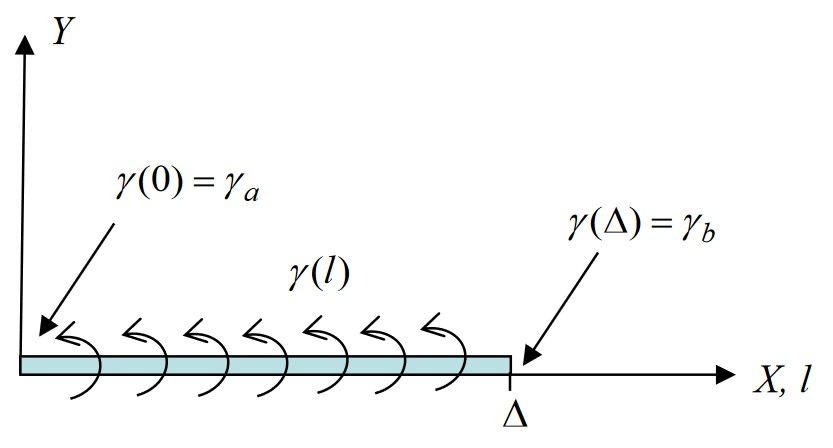
\includegraphics[width=0.3\textwidth]{figures/single_panel.jpg}
    \caption{Single Panel}
    \label{fig:single_panel}
\end{figure}
The streamfunction due to a linearly distributed vortex panel is given by
\begin{equation}
    \psi(X,Y) = \gamma_a f_a + \gamma_b f_b
\end{equation}
where $f_a$ and $f_b$ are influence coefficients of the panel at points $a$ and $b$ respectively.
The influence functions can be found by integrating the Biot-Savart law over the panel.
A function is written to calculate the influence coefficients for arbitrary panel points through coordinate transformations.

The streamfunction due to the superposition of all panels is given by
\begin{equation}
    \psi_p(x_i, y_i) = \sum_{\text{ip} = 1}^\text{np} \left[ \gamma_\text{ip} f_a^{(\text{ip})} + \gamma_{\text{ip}+1} f_b^{(\text{ip})} \right]
\end{equation}
This can be written in matrix format as $\psi_p(x_i, y_i) = \left[ \boldsymbol{\Psi \gamma} \right]_i$ and the overall streamfunction is $\psi = \psi_p + \psi_{fs}$. \\
The free stream function is given by $\psi_{fs} = y\cos \alpha - x\sin \alpha$.

The stream function must be constant from panel edge to panel edge.
\begin{equation}
    \sum_{\text{j} = 1}^{\text{np}+1} \left[  \boldsymbol{\Psi}_{i+1,j}  - \boldsymbol{\Psi}_{i,j} \right] \gamma_j = \psi_{fs}(x_i, y_i) - \psi_{fs}(x_{i+1}, y_{i+1})
\end{equation}
This can be written in matrix form as $ \mathbf{A} \boldsymbol{\gamma} = \boldsymbol{b}$ with
\begin{align}
    \mathbf{A}_{i,j} = \boldsymbol{\Psi}_{i+1,j} &- \boldsymbol{\Psi}_{i,j} \\
    \boldsymbol{b}_i = \psi_{fs}(x_i, y_i) &- \psi_{fs}(x_{i+1}, y_{i+1}) \\
\end{align}
The final equations are supplied by the repetition $\gamma_{\text{np}+1} = \gamma_1$ and the trailing edge Kutta condition $\gamma_{\text{np}+1} = -(u_e)_{\text{te}}$.
The trailing edge velocity is extrapolated from the last two panels.
\begin{equation}
    (u_e)_{\text{te}} = \gamma_2 - \frac{1}{2}\gamma_3 + \frac{1}{2}\gamma_{\text{np} - 1} - \gamma_{\text{np}}
\end{equation}

\subsection{Boundary Layer Solver}

From panel methods, the velocity distribution over the aerofoil surface is known.
From this the pressure distribution can be found and the boundary layer can be solved for.
This gives an estimated drag coefficient for skin friction of the aerofoil.
This method also assumes a smooth surface and so does not account for surface roughness.

The routine for solving the upper or lower aerofoil surface boundary layer is shown below in figure \ref{fig:BL}.
\begin{figure}[H]
    \centering
    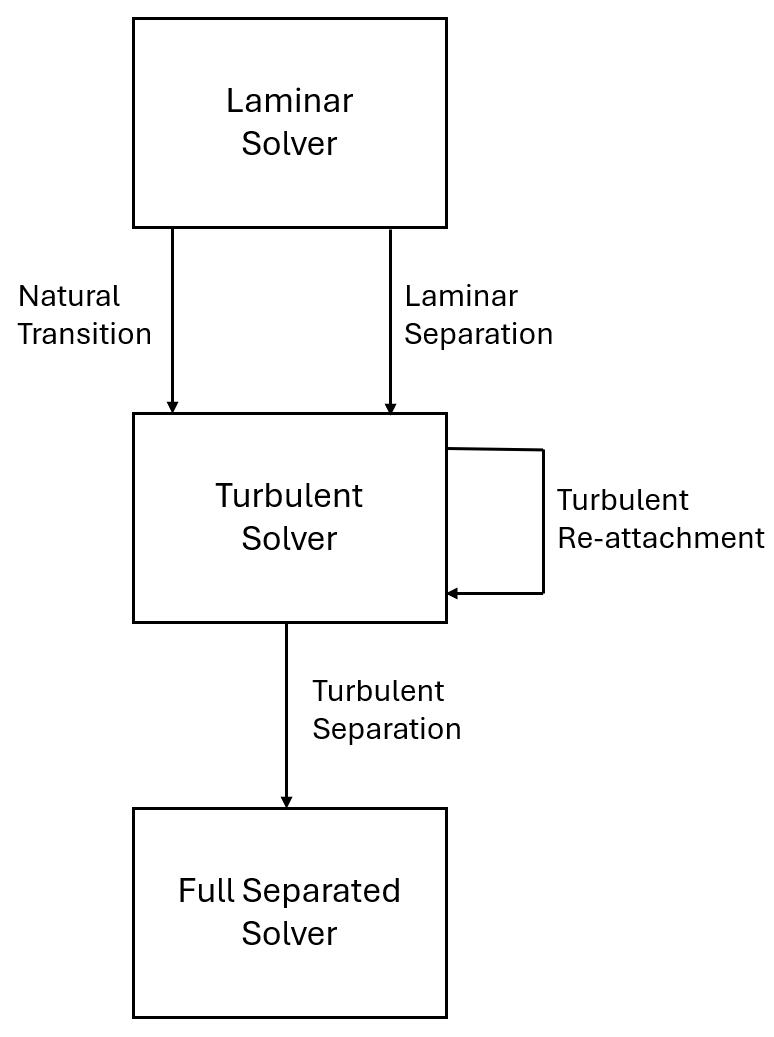
\includegraphics[width=0.3\textwidth]{figures/bl_solver_flowchart.png}
    \caption{Boundary Layer Solve Routine}
    \label{fig:BL}
\end{figure}
In box represents an iterative loop that is marches along the panels of the aerofoil for the given flow regime.
Each iteration performs checks for relevent transitions and seperations,
which if triggered sets an index flag and loops the new regime starting on the same panel.

\subsubsection{Laminar Regime}

For the laminar regime, Thwaites' solution is used to accelerate the calculation of the boundary layer profile.

\begin{equation}
    \ln(Re_\theta) = 18.4 H_E - 21.74 \quad \text{ where } \quad Re_\theta = Re_L\left( \frac{u_e}{U} \right) \left( \frac{\theta}{L} \right)
\end{equation}

Thwaites' method defines a form parameter $m$ that uniquely determines the shape of the velocity profile.
\begin{equation}
    m = - \frac{\theta^2}{\mu}\frac{du_e}{dx} = -Re_L \left( \frac{\theta}{L} \right)^2 \frac{d(u_e / U)}{d(x/L)}
    \label{}
\end{equation}
From the momentum integral equation it can be shown that
\begin{equation}
    U\frac{d}{dx}\left( \theta^2 \right) = 2\nu[m(H+2) + l] = \nu L(m)
\end{equation}
A general fit for $L(m)$ is given by $L(m) = 0.45 + 6m$, however for adverse pressure gradients this relation is poor
as in reality the profiles cannot be expressed simply in terms of one parameter, $m$ \cite{BL_notes}.
With this relation, the analytical Thwaites solution is found as
\begin{equation}
    \left[ \frac{\theta}{L}\right]^2 = \frac{0.45}{Re_L} \left[\frac{u_e(x)}{U} \right]^{-6} \int_0^{x/L} \left[ \frac{u_e(x')}{U} \right]^5 d \left( \frac{x'}{L} \right)
\end{equation}
The velocity is discretized at the panel edges and so is taken as linear over the panels.
The additional integral term for the panel behind the $i$th point is calculated using the equation below and is added to a cumulative sum variable.
\begin{equation}
    \int_{x_{i-1}}^{x_i} \left[ \frac{u_e(x')}{U} \right]^5 d \left( \frac{x'}{L} \right) = \left[ \bar{u}^5 + \frac{5}{6}(\Delta u)^2 + \frac{1}{16}(\Delta u)^5 \right] \Delta x
\end{equation}
where $\bar{u} = (u_{i} - u{i-1})/2$ and $\Delta u = u_i - u_{i-1}$.
Checks are made for laminar separation and transition to turbulent flow as seen in figure \ref{fig:BL}.

If $m > 0.09$, then the laminar boundary layer seperates and is treated as turbulent.
The shape factor can also be determined by a lookup table from $m$ and is used to test for natural transition to turbulent flow.
$H_E$ is found from $H$ from a given script \cite{handout} based on an inverted relation by Eppler and Somers \cite{Eppler_Somers}.
Natural transition is detected by the empirical criterion also proposed by Eppler and Somers \cite{Eppler_Somers}.
\begin{equation}
    \log{Re_\theta} = 18.4 H_E - 21.74 \quad \text{ where } \quad Re_\theta = Re_L\left( \frac{(u_e)_i}{U} \right) \left( \frac{\theta_i}{L} \right)
\end{equation}

\subsubsection{Turbulent Regime}

The turbulent regime cannot be solved analytically and so is solved numerically.
Von Karman's boundary-layer integral equation is given by
\begin{equation}
    \dot{\mathbf{y}} = \begin{bmatrix}
        \frac{d \theta}{d x} \\[5pt]
        \frac{d \delta_E}{d x}
    \end{bmatrix} = f(x,\mathbf{y}) = \begin{bmatrix}
        \frac{c_f}{2} - \frac{H+2}{u_e}\frac{d u_e}{d x} \theta \\[5pt]
        c_\text{diss} - \frac{3}{u_e} \frac{d \delta_E}{d x} \delta_E
    \end{bmatrix}
\end{equation}
Where $c_f$ and $c_\text{diss}$ are empirical relations for the skin friction coefficient and dissipation coefficient respectively.
Empirical relations for these coefficients and the shape factor proposed by Eppler and Somers \cite{Eppler_Somers} are used.
\begin{align}
    H &= \begin{cases}
        \frac{11 H_E + 15}{48H_E - 59} & \text{if } H_E  \ge 1.46 \\
        2.803 & \text{if } H_E < 1.46
    \end{cases} \\
    c_f &= 0.091416\left[(H-1)Re_\theta \right]^{-0.232}e^{-1.26H} \\
    c_\text{diss} &= 0.010024\left[(H-1)Re_\theta \right]^{1/6}
\end{align}

A test for turbulent transition is made by calculating the new panels energy shape factor and comparing it to the critical
value proposed by Eppler and Somers $H_E < 1.46$ \cite{Eppler_Somers}.

\subsubsection{Complete Separation}

After turbulent separation, it is assumed that the shape factor remains unchanged from its seperation value.

\begin{equation}
    \theta_{i} = \theta_{i-1} \left( \frac{(u_e)_{i-1}}{(u_e)_i} \right) ^ {(H + 2)}
\end{equation}


\section{Software Performance}

\subsection{Comparison with Experimental Data}

\begin{figure}[H]
    \centering
    \captionsetup{justification=centering}
    \begin{subfigure}{0.45\textwidth}
        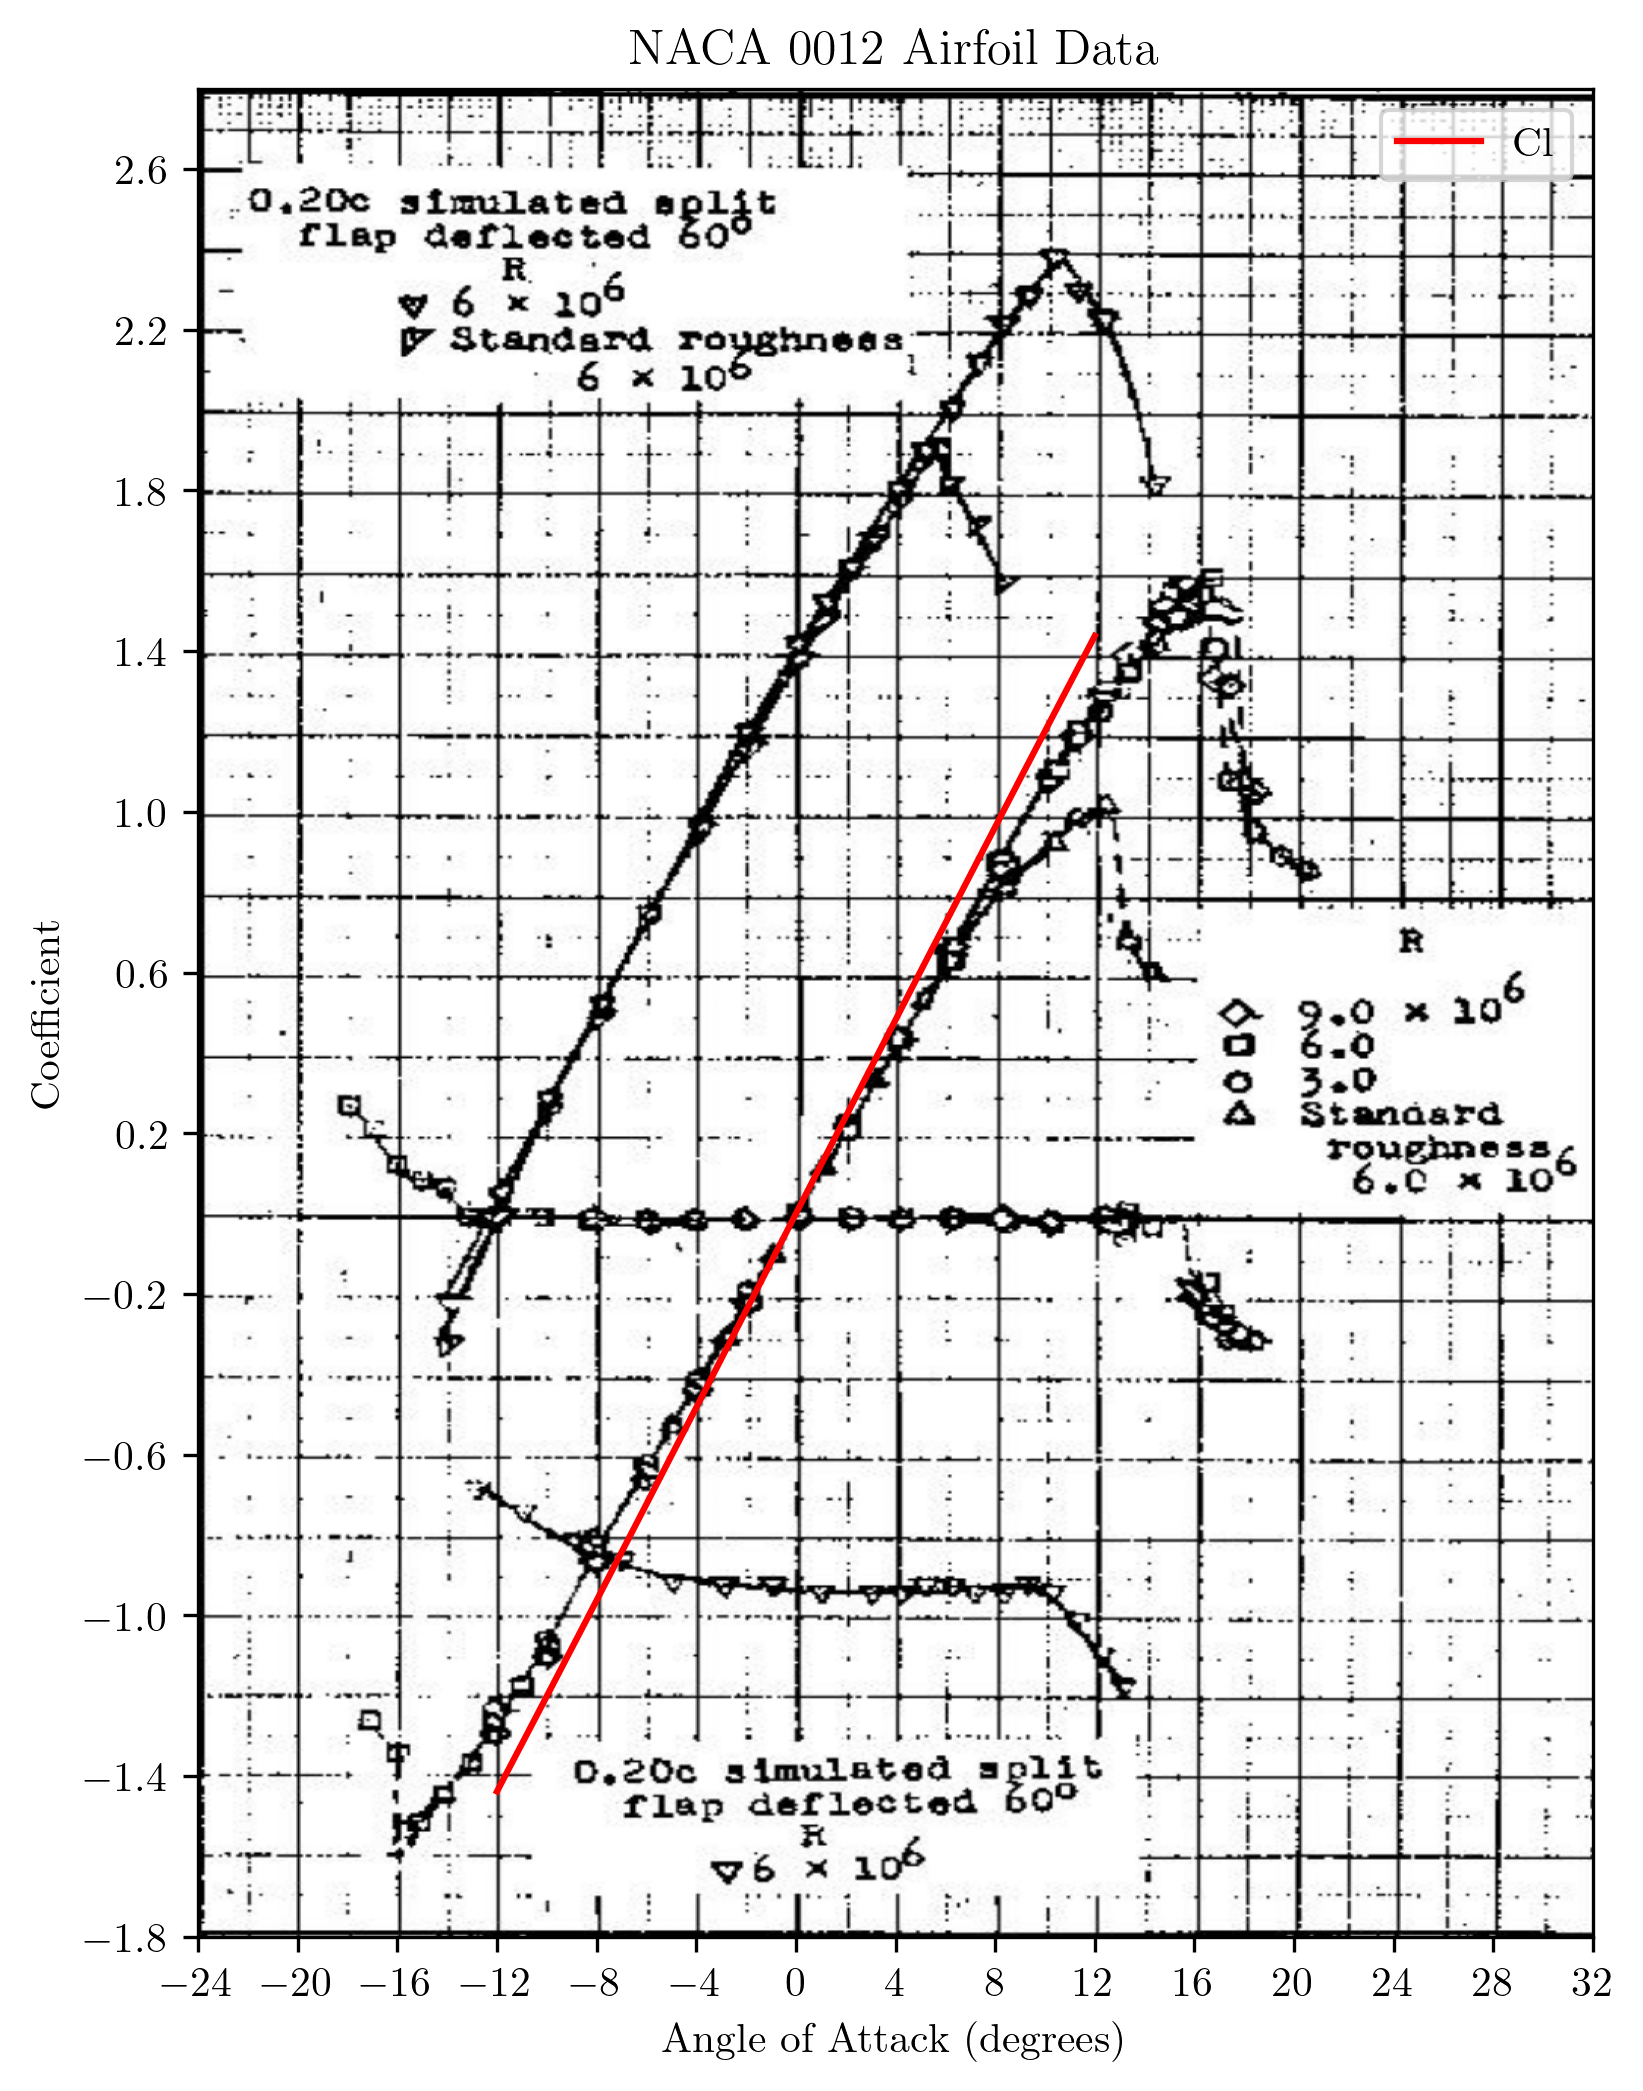
\includegraphics[width=0.99\textwidth]{figures/NACA0012_lift_validation.png}
        \caption{Lift coefficient against angle of attack}
        \label{fig:0012_lift_validation}
    \end{subfigure}
    \begin{subfigure}{0.45\textwidth}
        \centering
        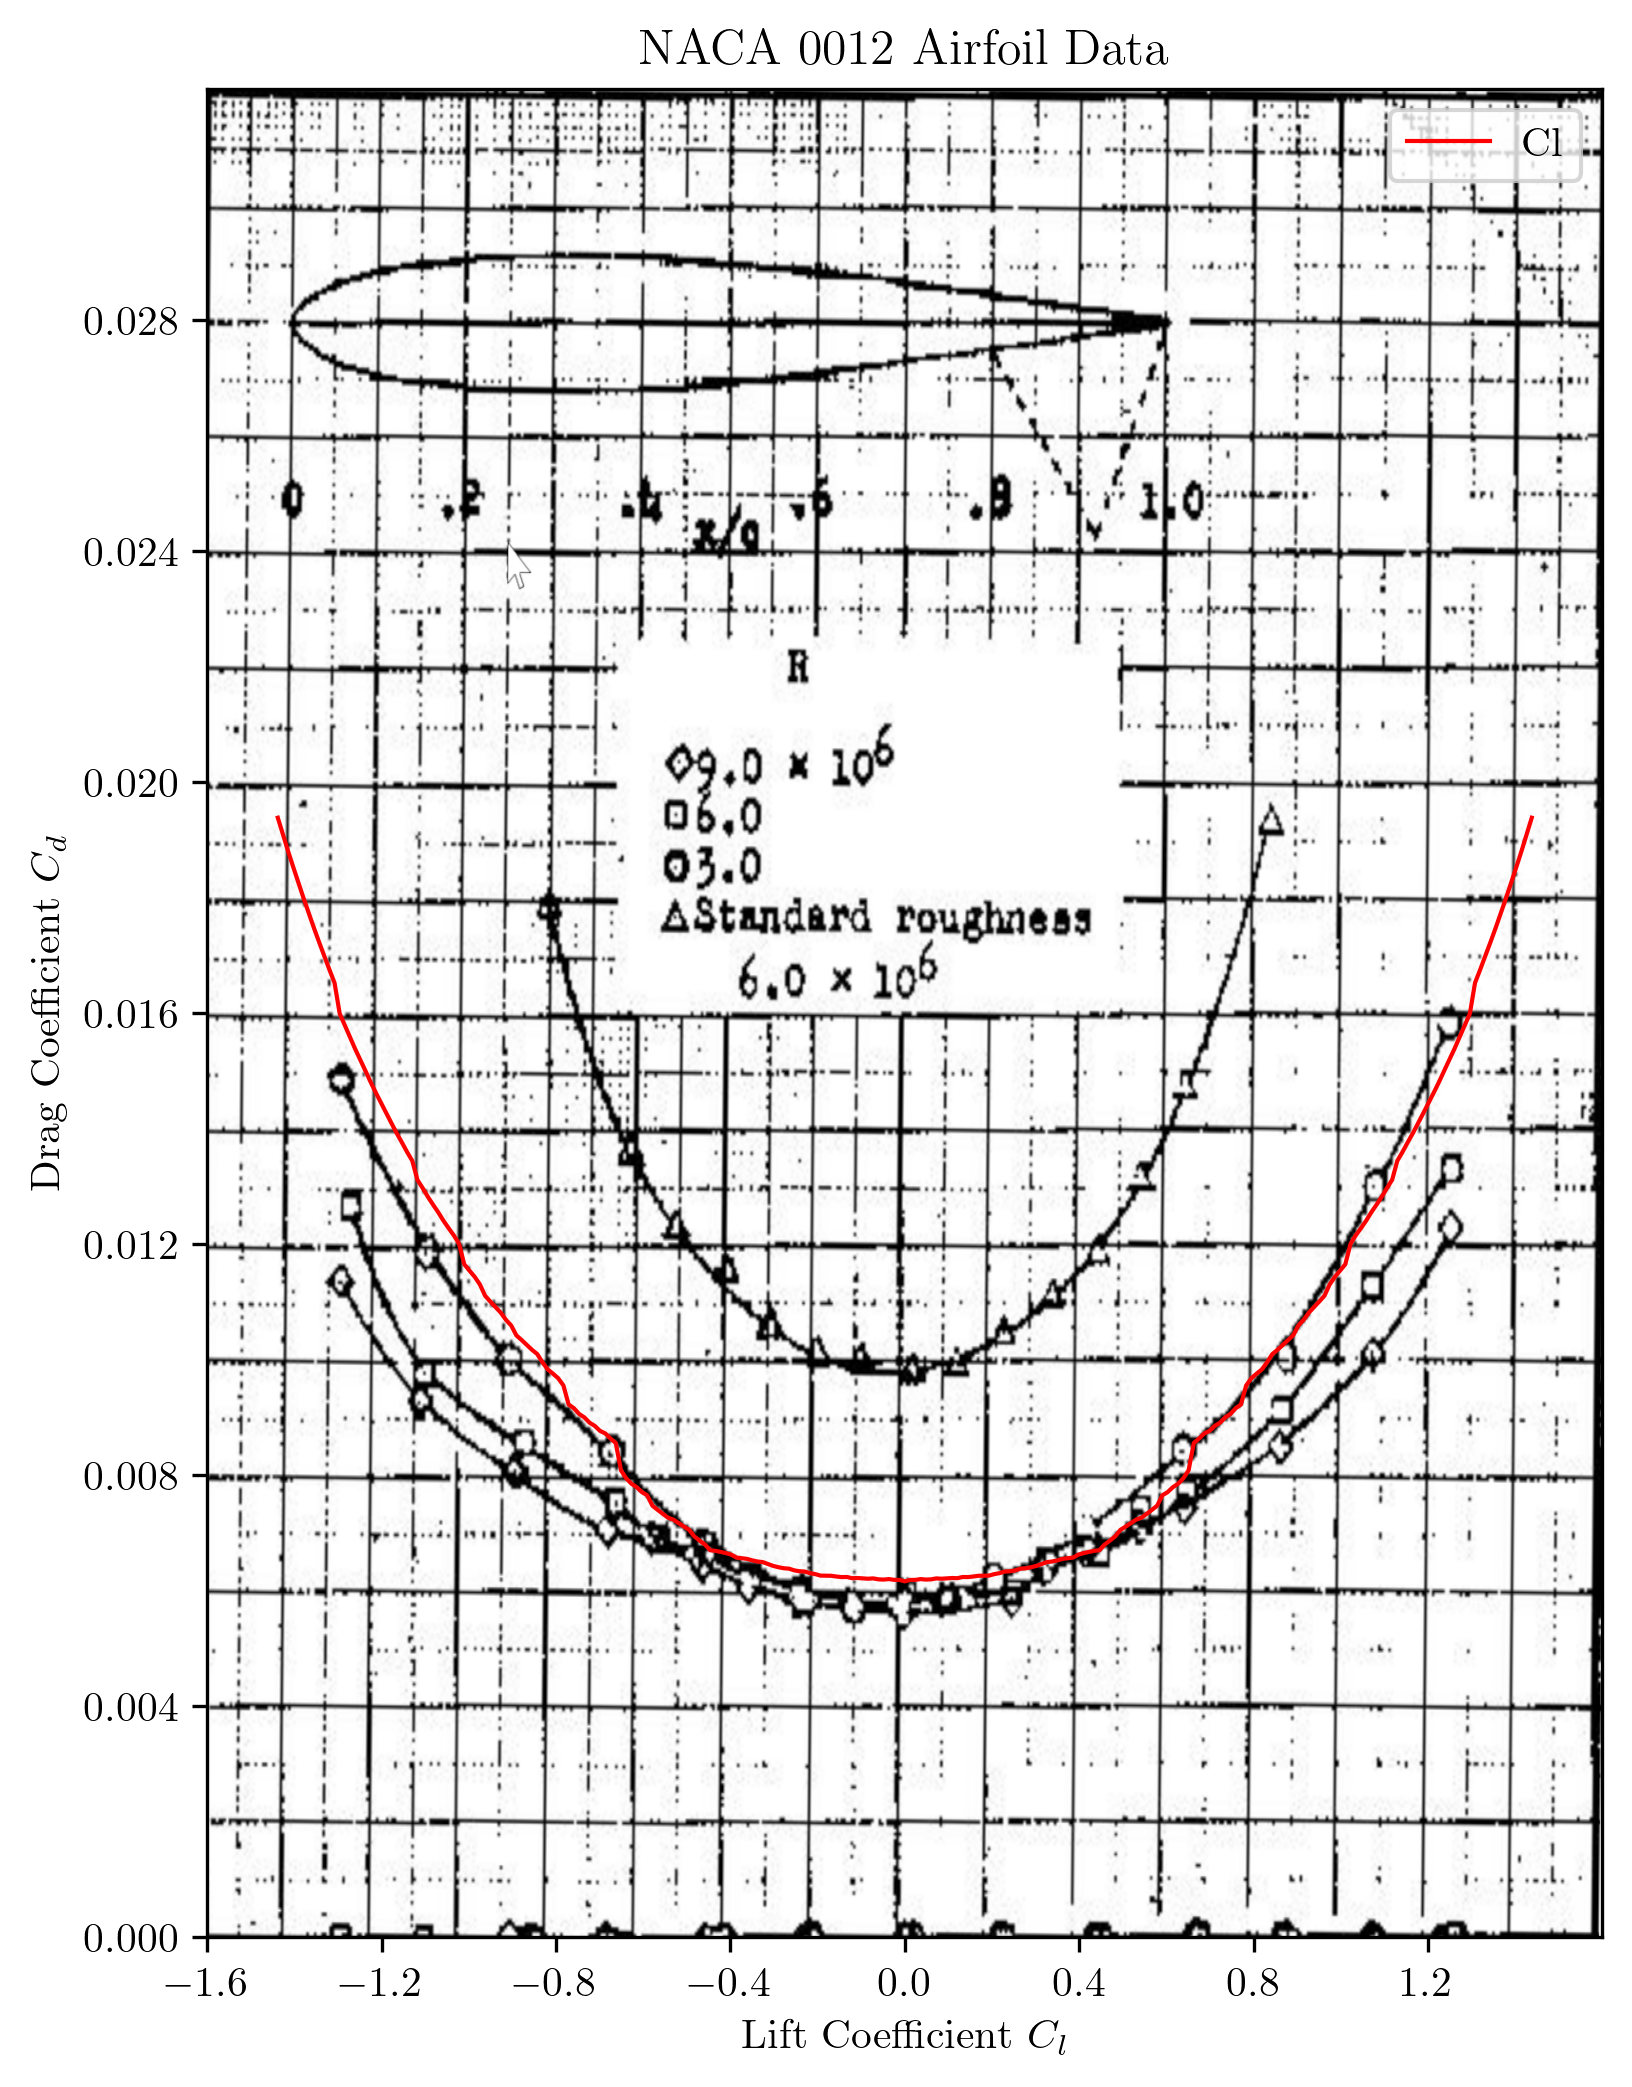
\includegraphics[width=0.99\textwidth]{figures/NACA0012_drag_validation.png}
        \caption{Drag coefficient against lift coefficient}
        \label{fig:0012_drag_validation}
    \end{subfigure}
    \caption{Experimetnal and calculated performance at $Re = 3\times10^6$ for the NACA0012 aerofoil}
\end{figure}

\begin{figure}[H]
    \centering
    \captionsetup{justification=centering}
    \begin{subfigure}{0.45\textwidth}
        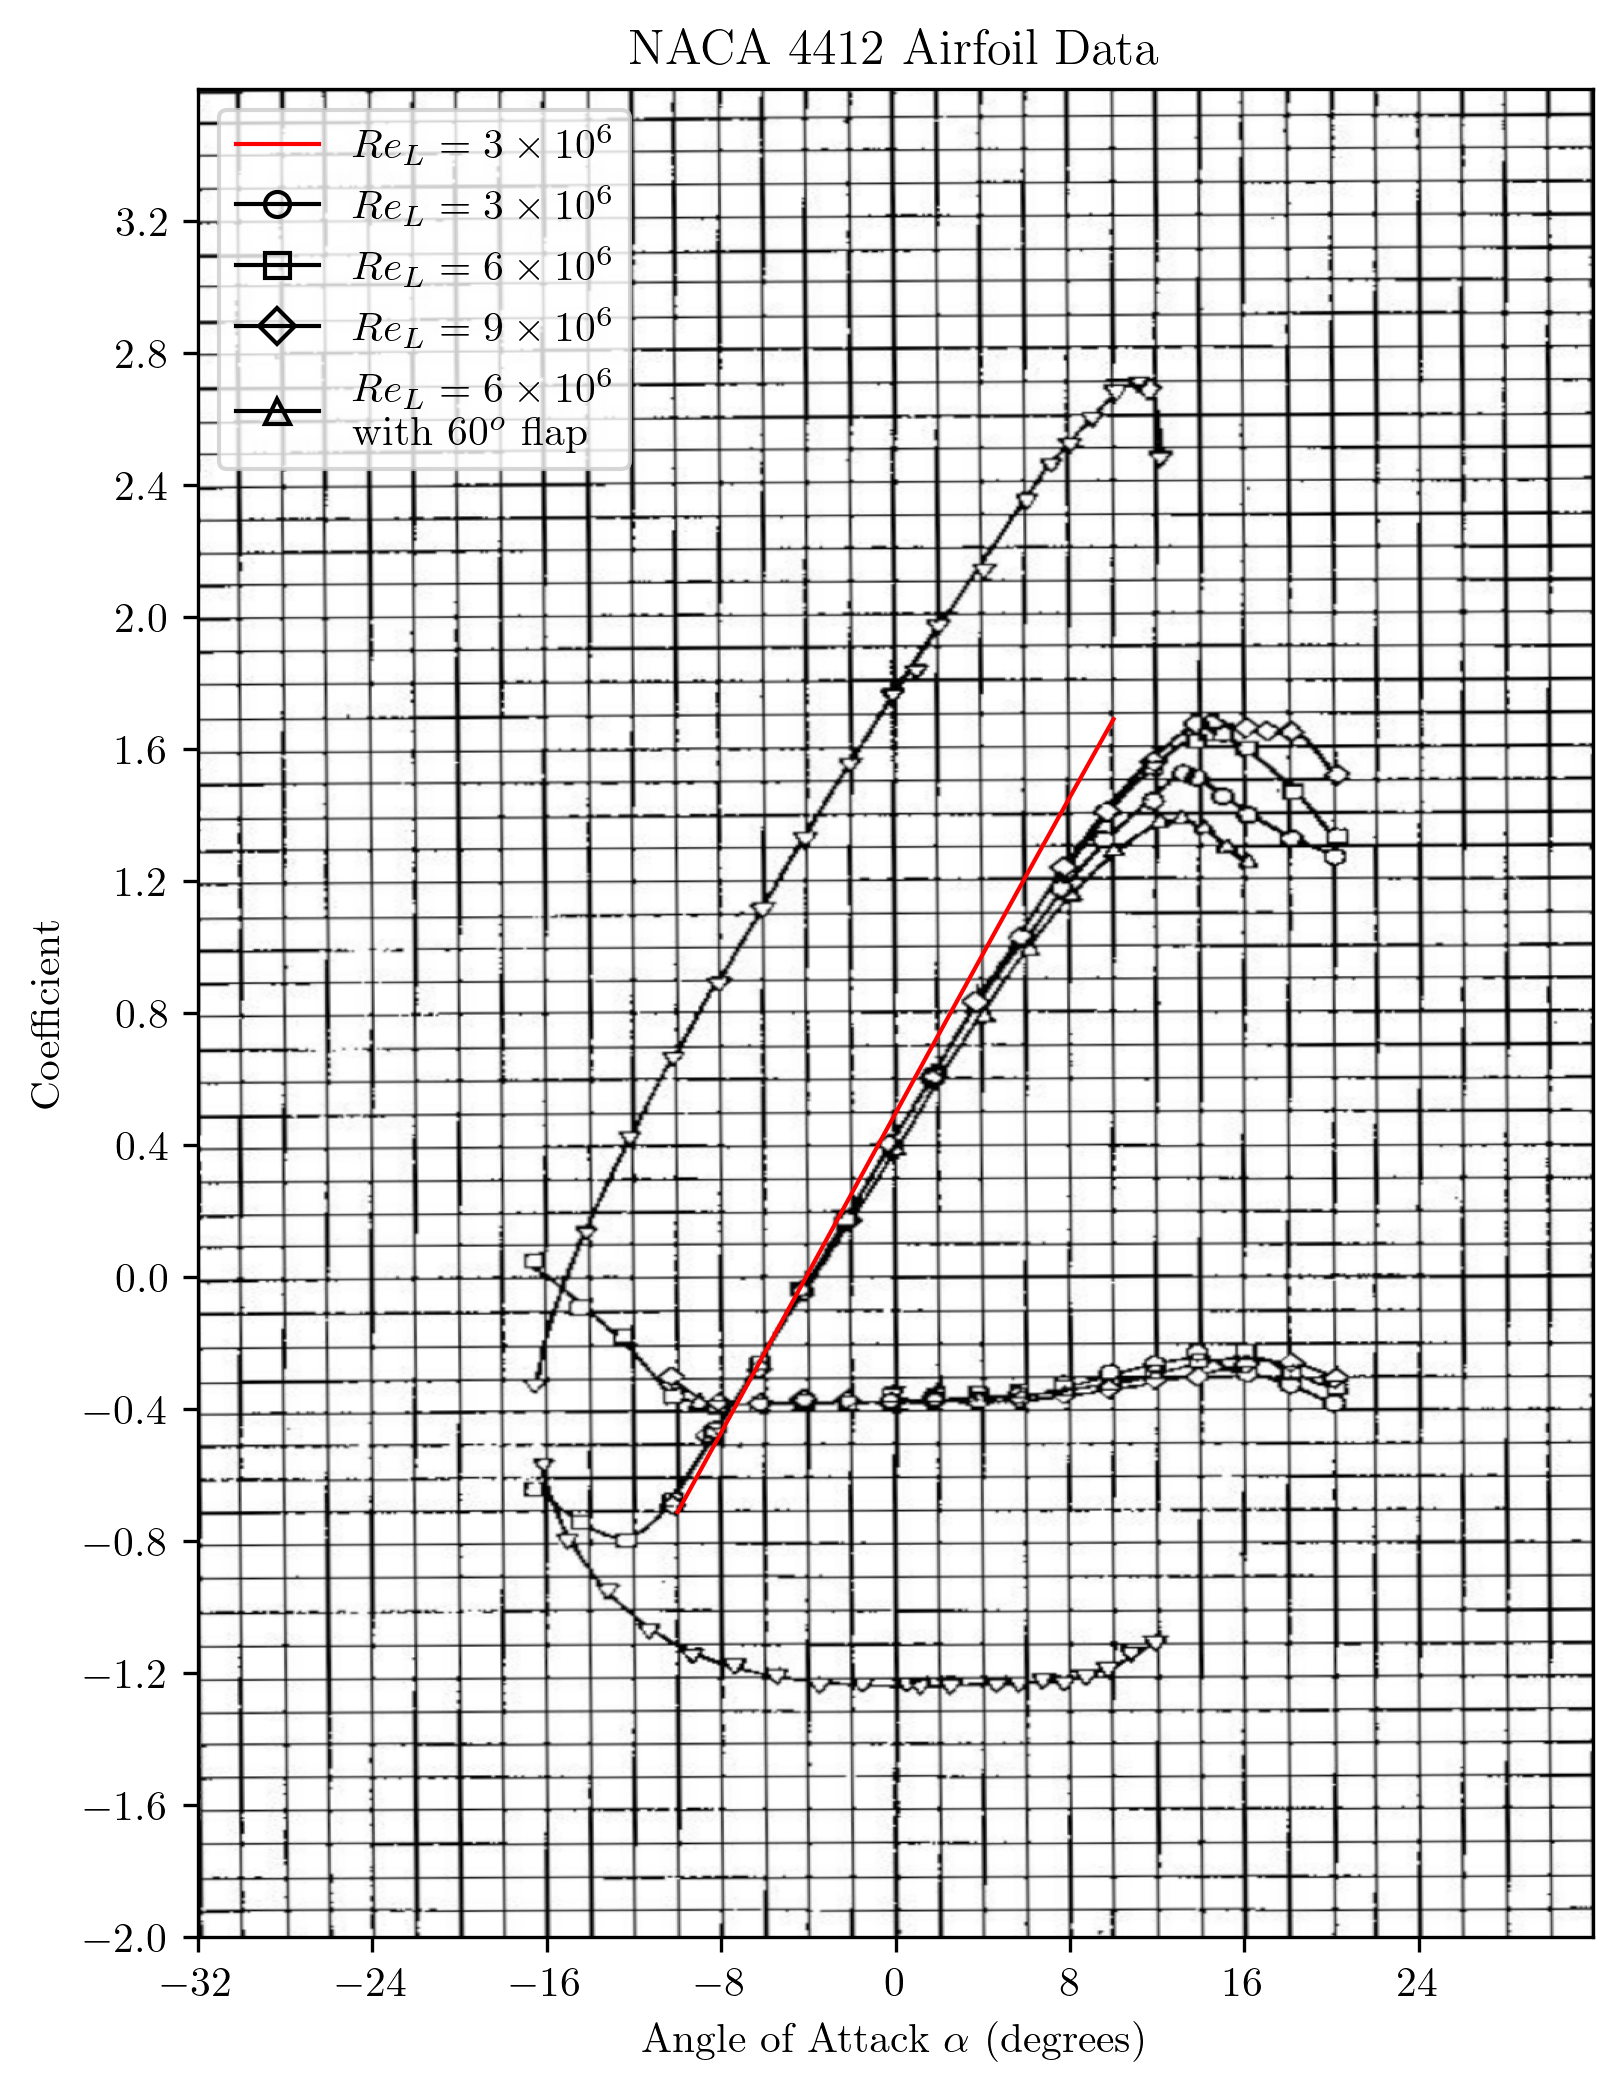
\includegraphics[width=0.9\textwidth]{figures/NACA4412_lift_validation.png}
        \caption{Lift coefficient against angle of attack}
        \label{fig:4412_lift_validation}
    \end{subfigure}
    \begin{subfigure}{0.45\textwidth}
        \centering
        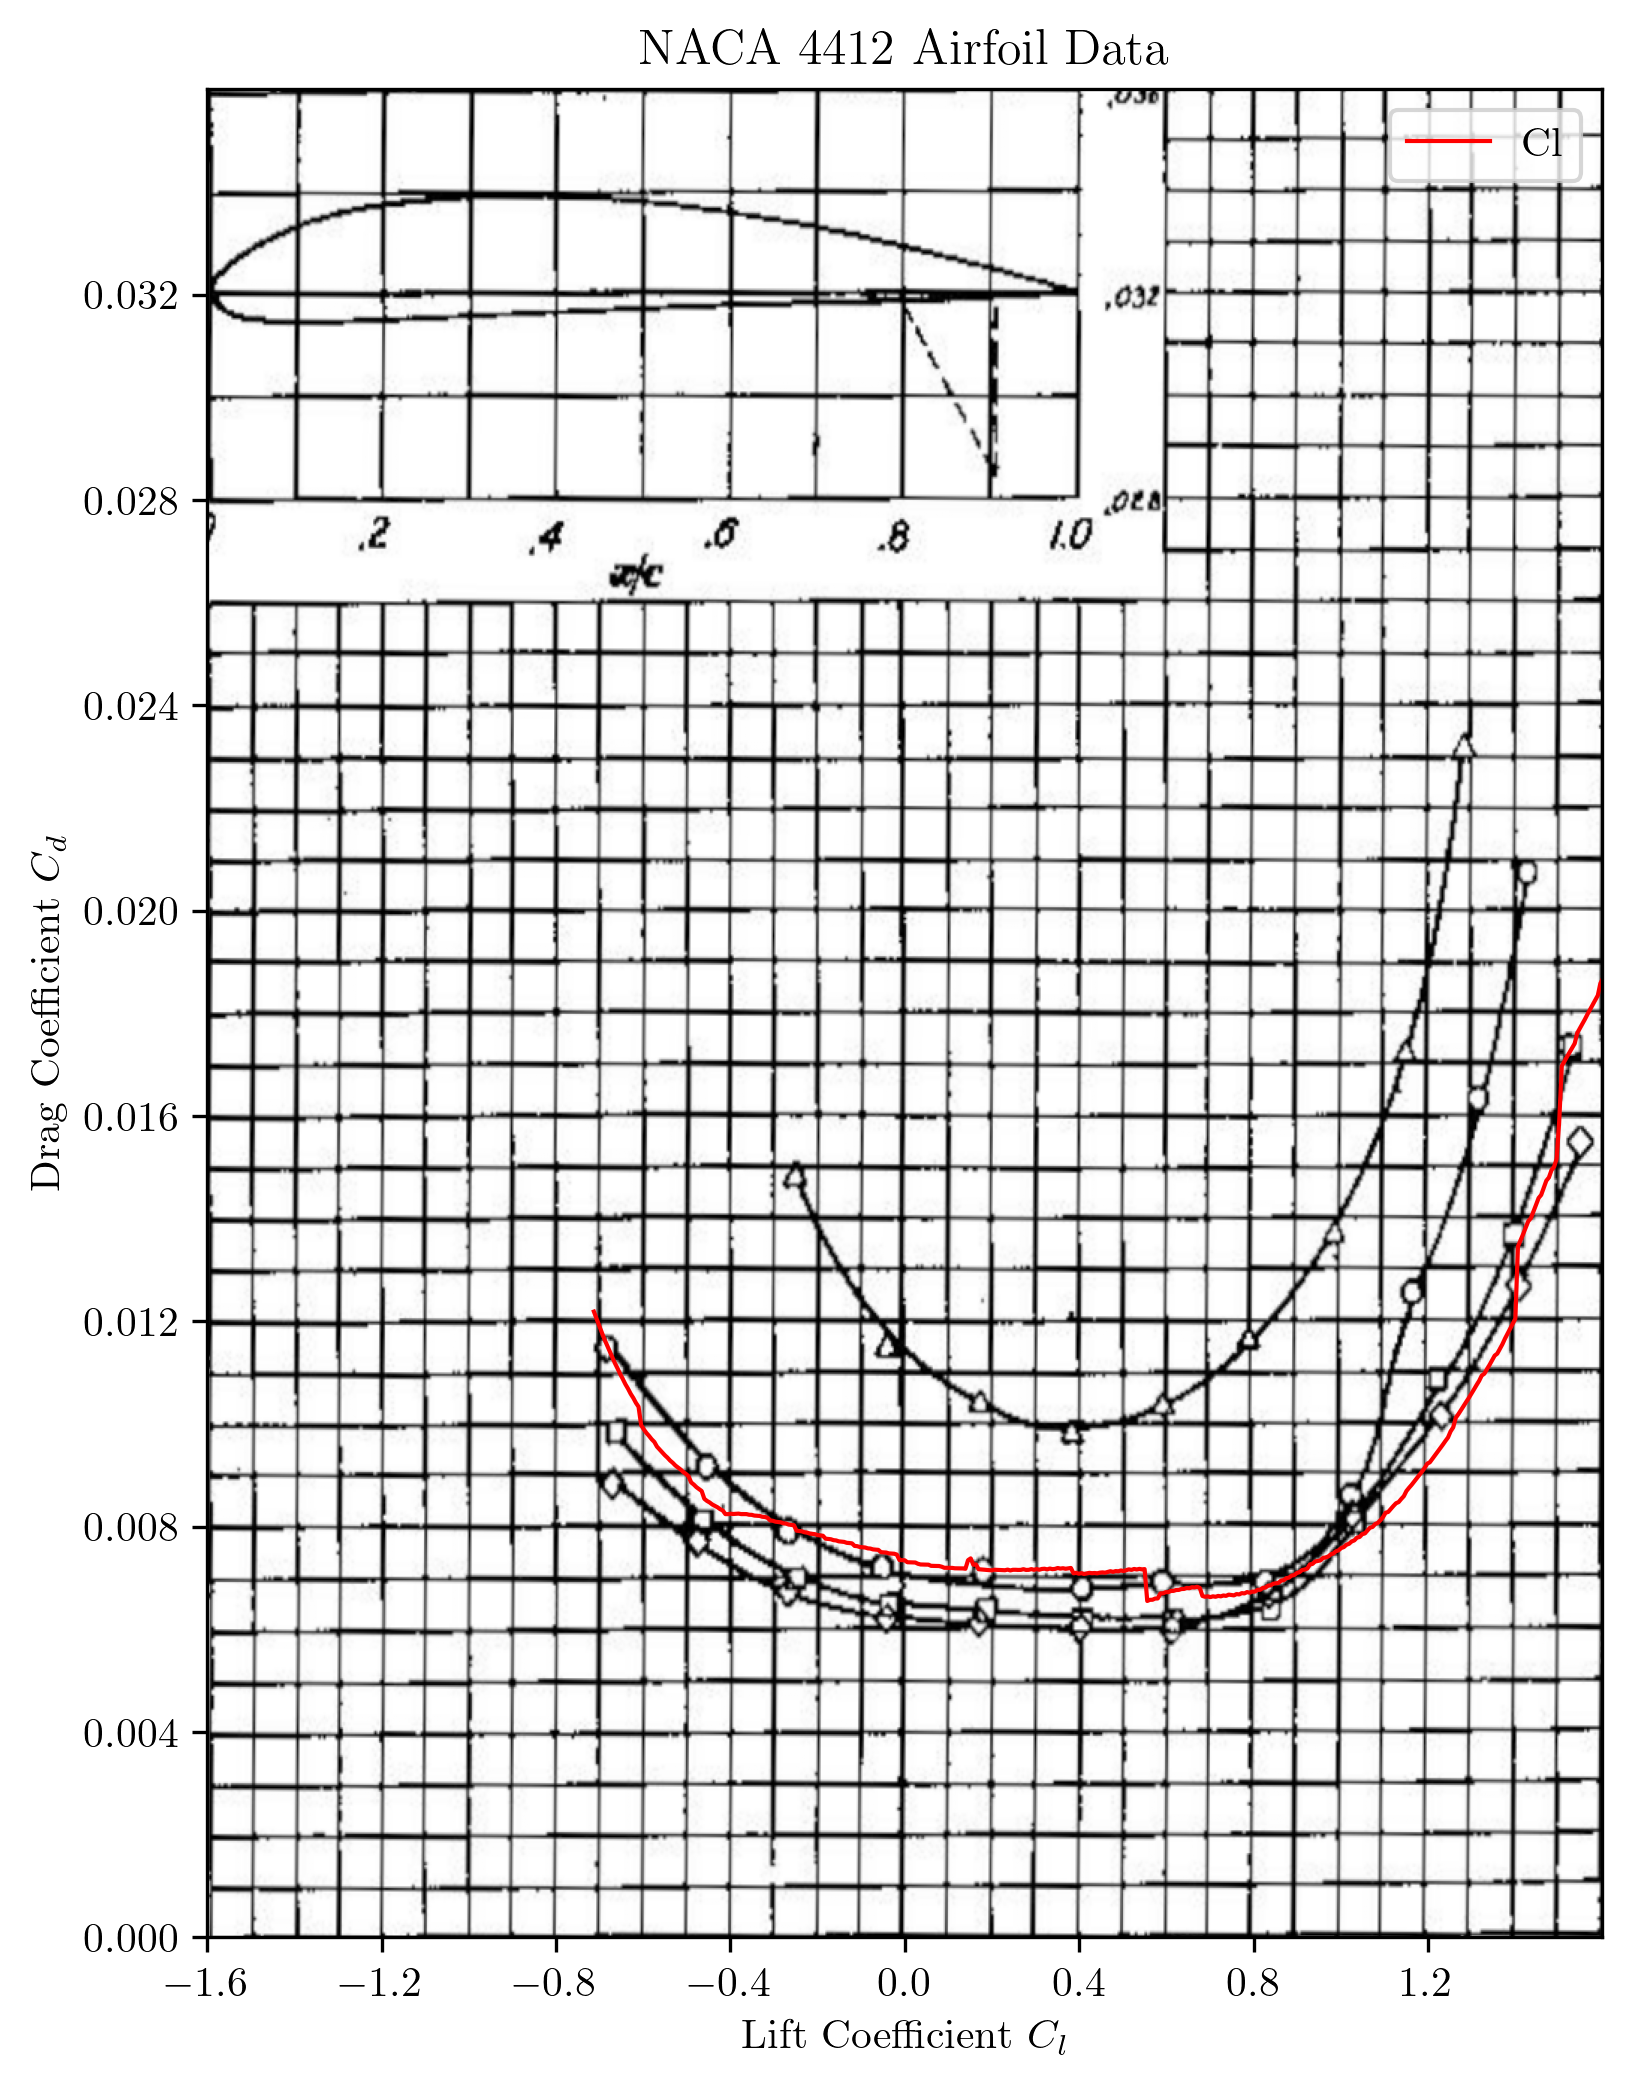
\includegraphics[width=0.9\textwidth]{figures/NACA4412_drag_validation.png}
        \caption{Drag coefficient against lift coefficient}
        \label{fig:4412_drag_validation}
    \end{subfigure}
    \caption{Experimetnal and calculated performance at $Re = 3\times10^6$ for the NACA4412 aerofoil}
\end{figure}

\subsection{Discussion of limitations}

% 1. is only for 2D infinite length wings
% 2. subsonic flow only
% 2. discrete panel method - problems 
% talk about natural transition
% less known about seperations and reattachment but assume these are valid
% 3. unable to handle turbulent reattachment
% 4. does not account for surface roughness

\begin{itemize}
    \item The software is only valid for 2D infinite length wings. This neglects the effects of wing tip vortices and 3D effects.
    \item The software is only valid for subsonic flow conditions and does not account for compressibility effects. This limits the software to low speed applications.
    \item The discrete panel method used can lead to numerical errors and instabilities that are unphysical.
    \item The software assumes that the empirical relations used for laminar separation and turbulent reattachment are valid. However turbulent reattachment is not implemented which can occur some rare flow conditions.
    \item The boundary layer solver assumes a smooth aerofoil surface 
\end{itemize}

\section{Topology Optimization}

\subsection{Changing Topology}

A spline fit tool is used to paramaterize complex curves with a small number of control points.
The calculated lift and drag coefficients are very sensitive to control point position.

A Naca 0012 airfoil is used as a starting point to gain insight into the effect of changing the airfoil shape on performance.

\subsection{Objective}

The objective is to maximize the lift to drag ratio of the airfoil at a range of angles of attack.
It is important to consider a range of angles of attack for the airfoil for robust performance.
This is especially important for 3D wings as it ensures that tip stall is less likely for twist distrubtions from lifting line theory.

Two Reynolds numbers are considered, $Re = 20\times10^6$ and $Re = 5\times10^5$


\subsection{High Reynolds Number}

The first changes made to the initial NACA 0012 airfoil were increasing curvature of the top surface.
This was done first all along the airfoil, then only in the region of the leading edge.
This can be seen below in figure \ref{fig:v5_geometry} and the performance in figure \ref{fig:v5_lod}.

\begin{figure}[H]
    \centering
    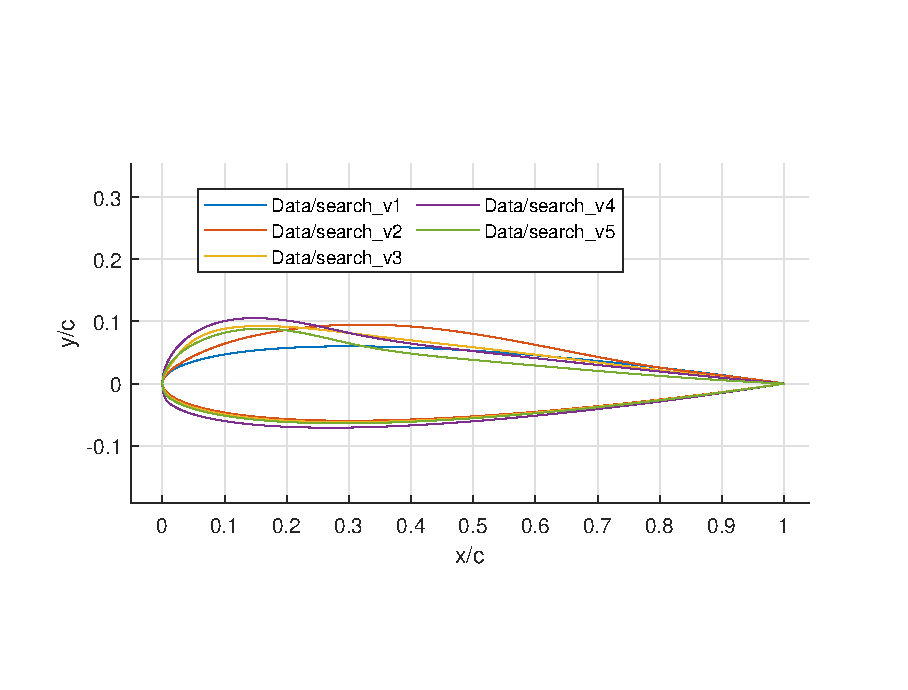
\includegraphics[width=0.8\textwidth]{figures/hiRe_geometry_5.eps}
    \caption{Airfoil Geometry of first 5 design iterations}
    \label{fig:v5_geometry}
\end{figure}

\begin{figure}[H]
    \centering
    \begin{subfigure}{0.45\textwidth}
        \centering
        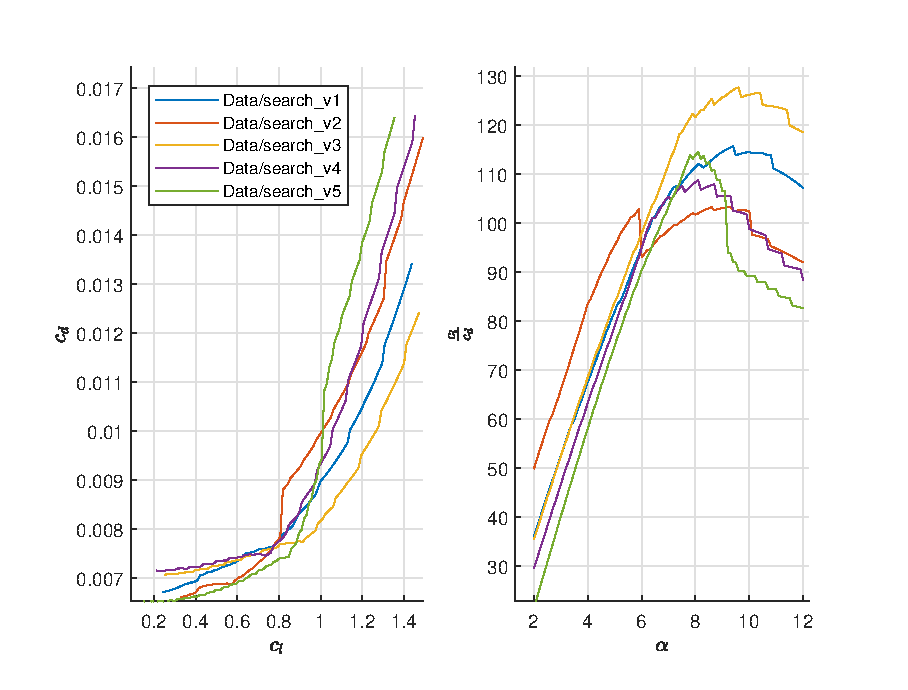
\includegraphics[width=1.2\textwidth, center]{figures/hiRe_lod_5.eps}
        \caption{Airfoil}
        \label{fig:v5_lod}
    \end{subfigure}
    \begin{subfigure}{0.54\textwidth}
        \centering
        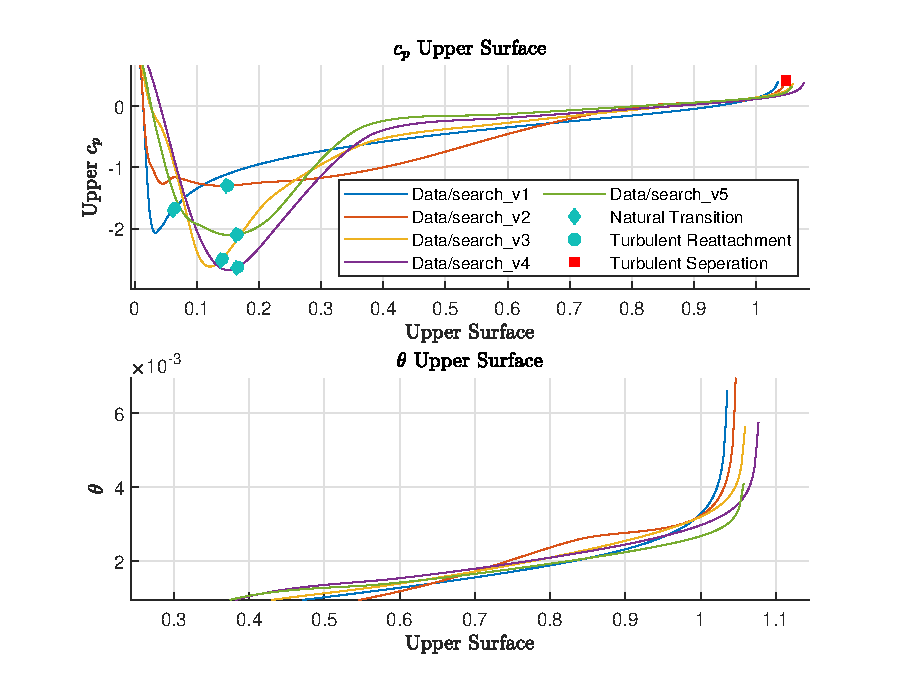
\includegraphics[width=0.99\textwidth]{figures/hiRe_upperprofile_5_a5.eps}
        \caption{Pressure coefficient and momentum thickness profiles for $\alpha = 5^\circ$}
        \label{fig:v5_uprofile}
    \end{subfigure}
    \caption{Performance of initial 5 design iterations and their upper surface boundary layer profiles}
\end{figure}

Figure \ref{fig:v5_uprofile} shows that these changes have a significant effect on the shape of the suction peak.
For maximum lift the area enclosed by the upper surface pressure coefficient profile should be minimised.
This means that the suction peak area should be maximised.
Version 2 had a 10\% higher lift coefficient which resulted in a higher lift to drag ratio seen in figure \ref{fig:v5_lod}.
All of versions 3 4 and 5 consisted of variations of the leading edge curvature which had worse lift to drag ratios.
This did move the suction peak further back along the upper surface but due to an increased gradient behind the peak,
the area enclosed by the profile was decreased overall.
A thinner version 5 produced a lift coefficient 11\% lower than the initial NACA 0012 airfoil.

Changes were then made to upper surface to ensure its convex to prevent adverse pressure gradients and increase area enclosed by the suction peak.
This can be seen in figure \ref{fig:v9_geometry} and the performance in figure \ref{fig:v9_lad}.

\begin{figure}[H]
    \centering
    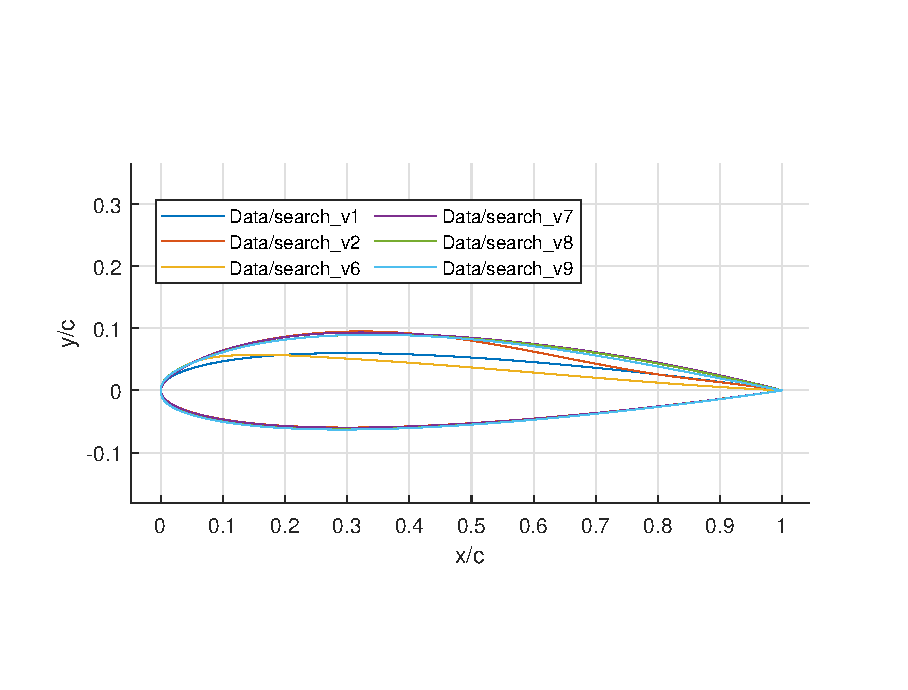
\includegraphics[width=0.8\textwidth]{figures/hiRe_geometry_9.eps}
    \caption{Airfoil Geometry}
    \label{fig:v9_geometry}
\end{figure}

\begin{figure}[H]
    \centering
    \begin{subfigure}{0.45\textwidth}
        \centering
        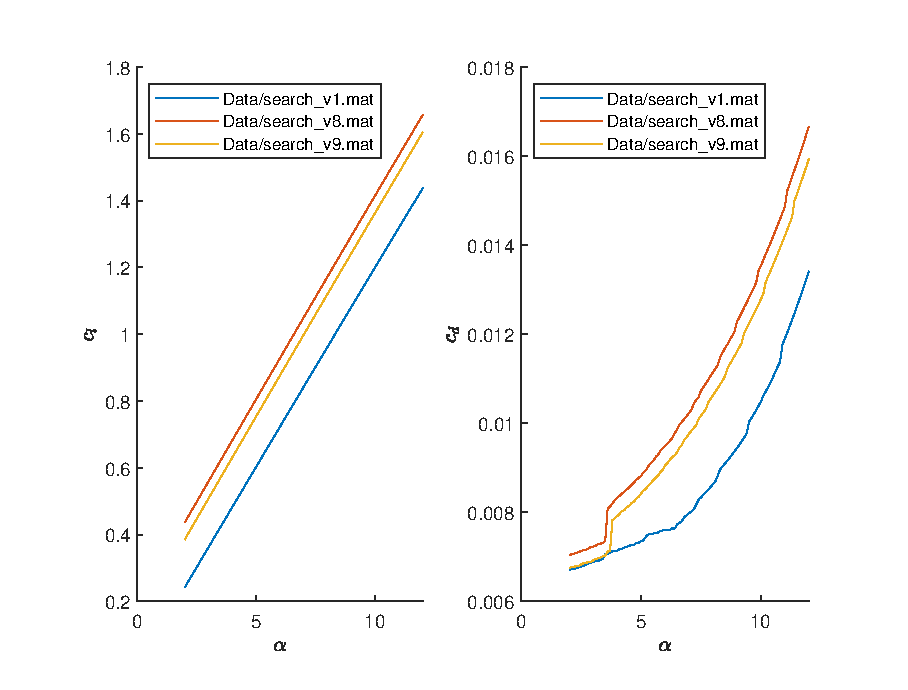
\includegraphics[width=1.2\textwidth, center]{figures/hiRe_lad_9.eps}
        \caption{Airfoil}
        \label{fig:v9_lad}
    \end{subfigure}
    \begin{subfigure}{0.54\textwidth}
        \centering
        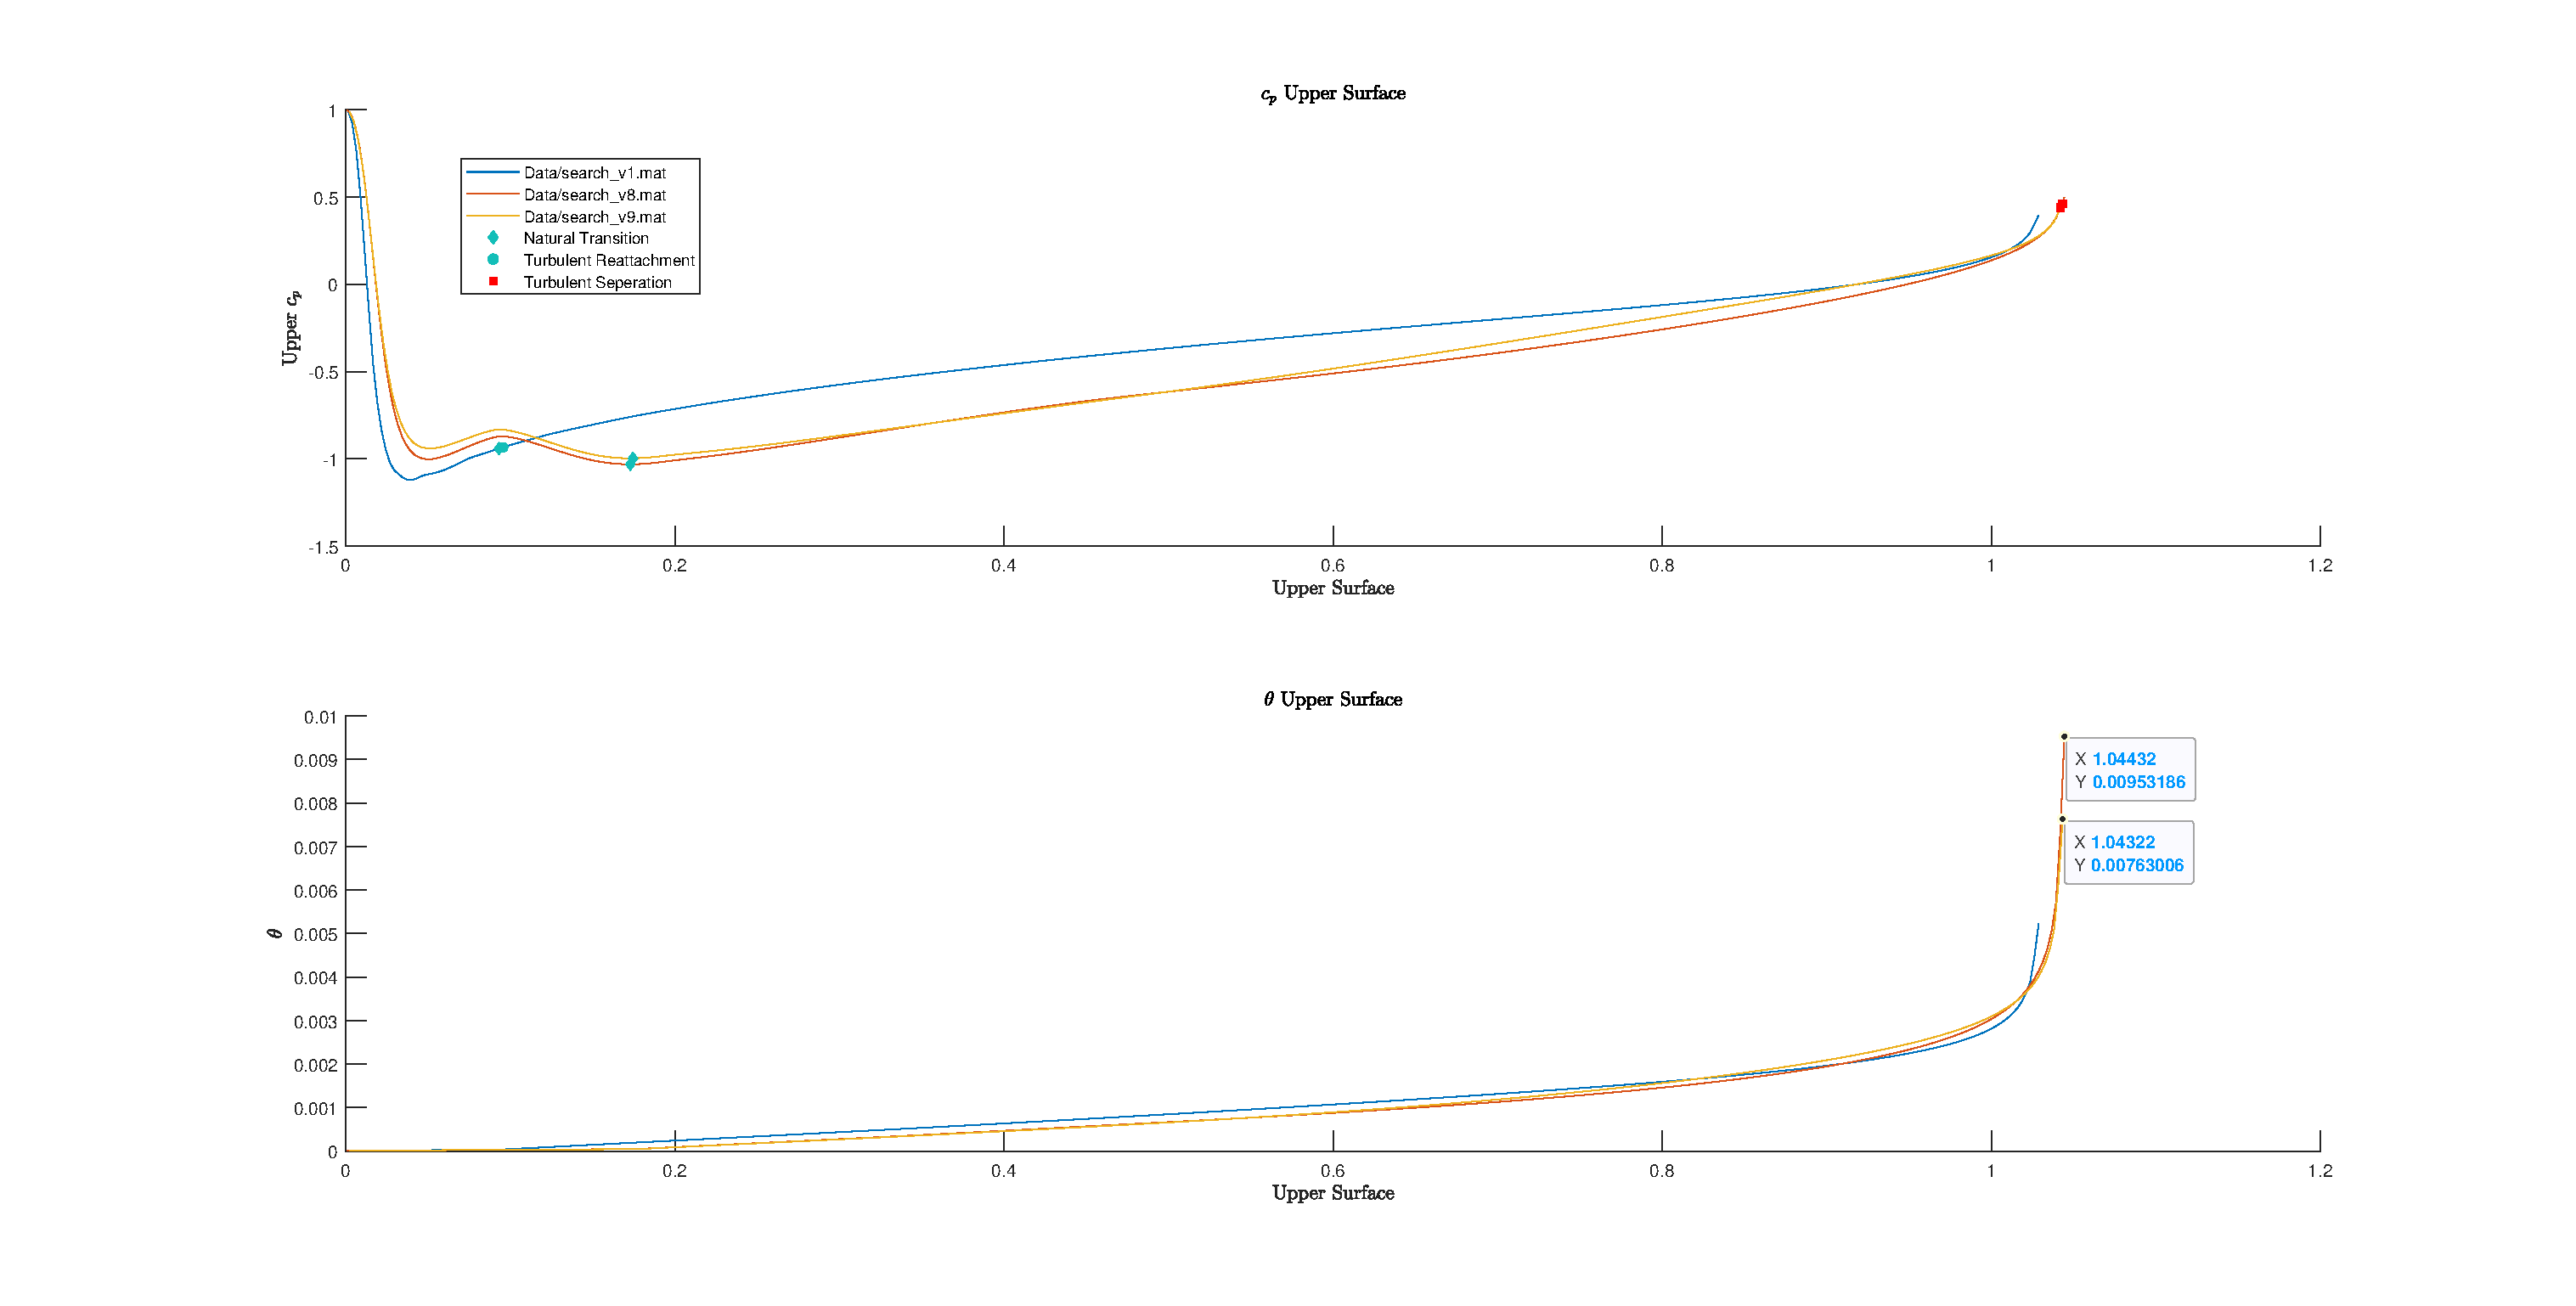
\includegraphics[width=0.99\textwidth]{figures/hiRe_upperprofile_9_a3.eps}
        \caption{Pressure coefficient and momentum thickness profiles for $\alpha = 3^\circ$}
        \label{fig:v9_uprofile}
    \end{subfigure}
    \caption{Performance of design iterations 6-9 and their upper surface boundary layer profiles}
\end{figure}

This change shows a higher lift achieved as the low pressure coefficient is maintained by the convex upper surface.
The drag coefficient curves for many designs in figure \ref{fig:v9_lad} show a sudden increase at varying angles of attack.
This is due to the point of transition to turbulence jumping forward on the upper surface with the increased angle of attack.
An earlier transition point means that the boundary layer can grow to be significantly thicker, increasing the drag of the aerofoil.
However, the NACA0012 demonstrates that early transition with small adverse pressure gradients can also produce lower drag coefficients.

Attempts were made to smooth the upper surface to prevent jumps in the transition point for a robust aerofoil design.
These can occur if there are too many closely spaced control points which can create a zig-zag shape, producing alternating favourable and adverse pressure gradients.
Small variations increasing the radius of curvature produced an even larger enclosed area by the suction peak and hence higher lift,
but at the cost of an increased pressure gradient behind the peak and hence higher drag (Versions 7 and 8).

Changes to the lower surface were then considered.
The lower surface was flattened to remove the adverse pressure gradient and increase pressure coefficient on the bottom surface to increase lift.

\begin{figure}[H]
    \begin{subfigure}{0.54\textwidth}
        \centering
        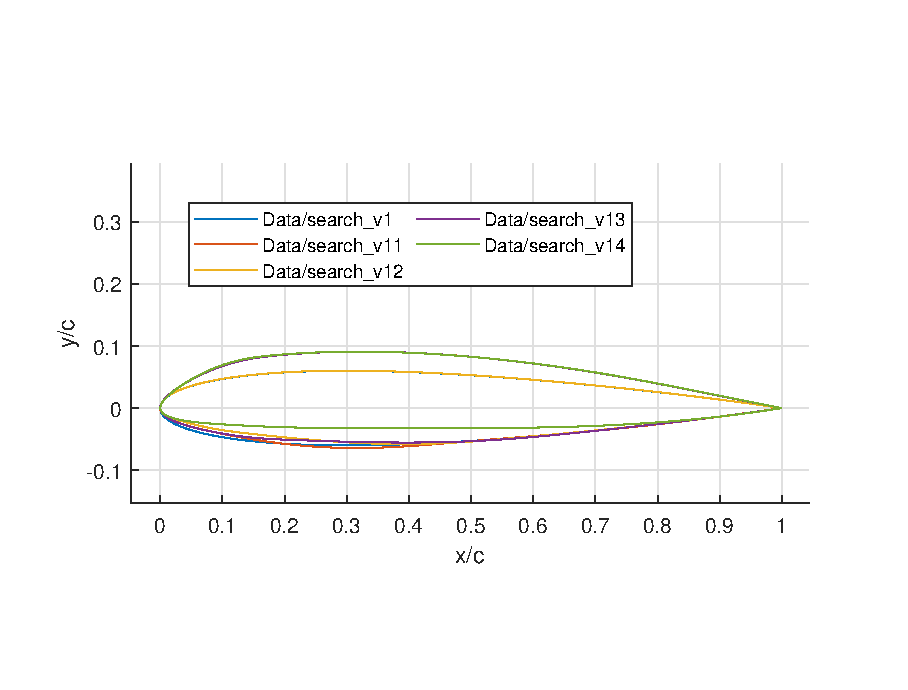
\includegraphics[width=1.2\textwidth, center]{figures/hiRe_geometry_14.eps}
        \caption{Airfoil Geometry}
        \label{fig:v14_geometry}
    \end{subfigure}
    \begin{subfigure}{0.45\textwidth}
        \centering
        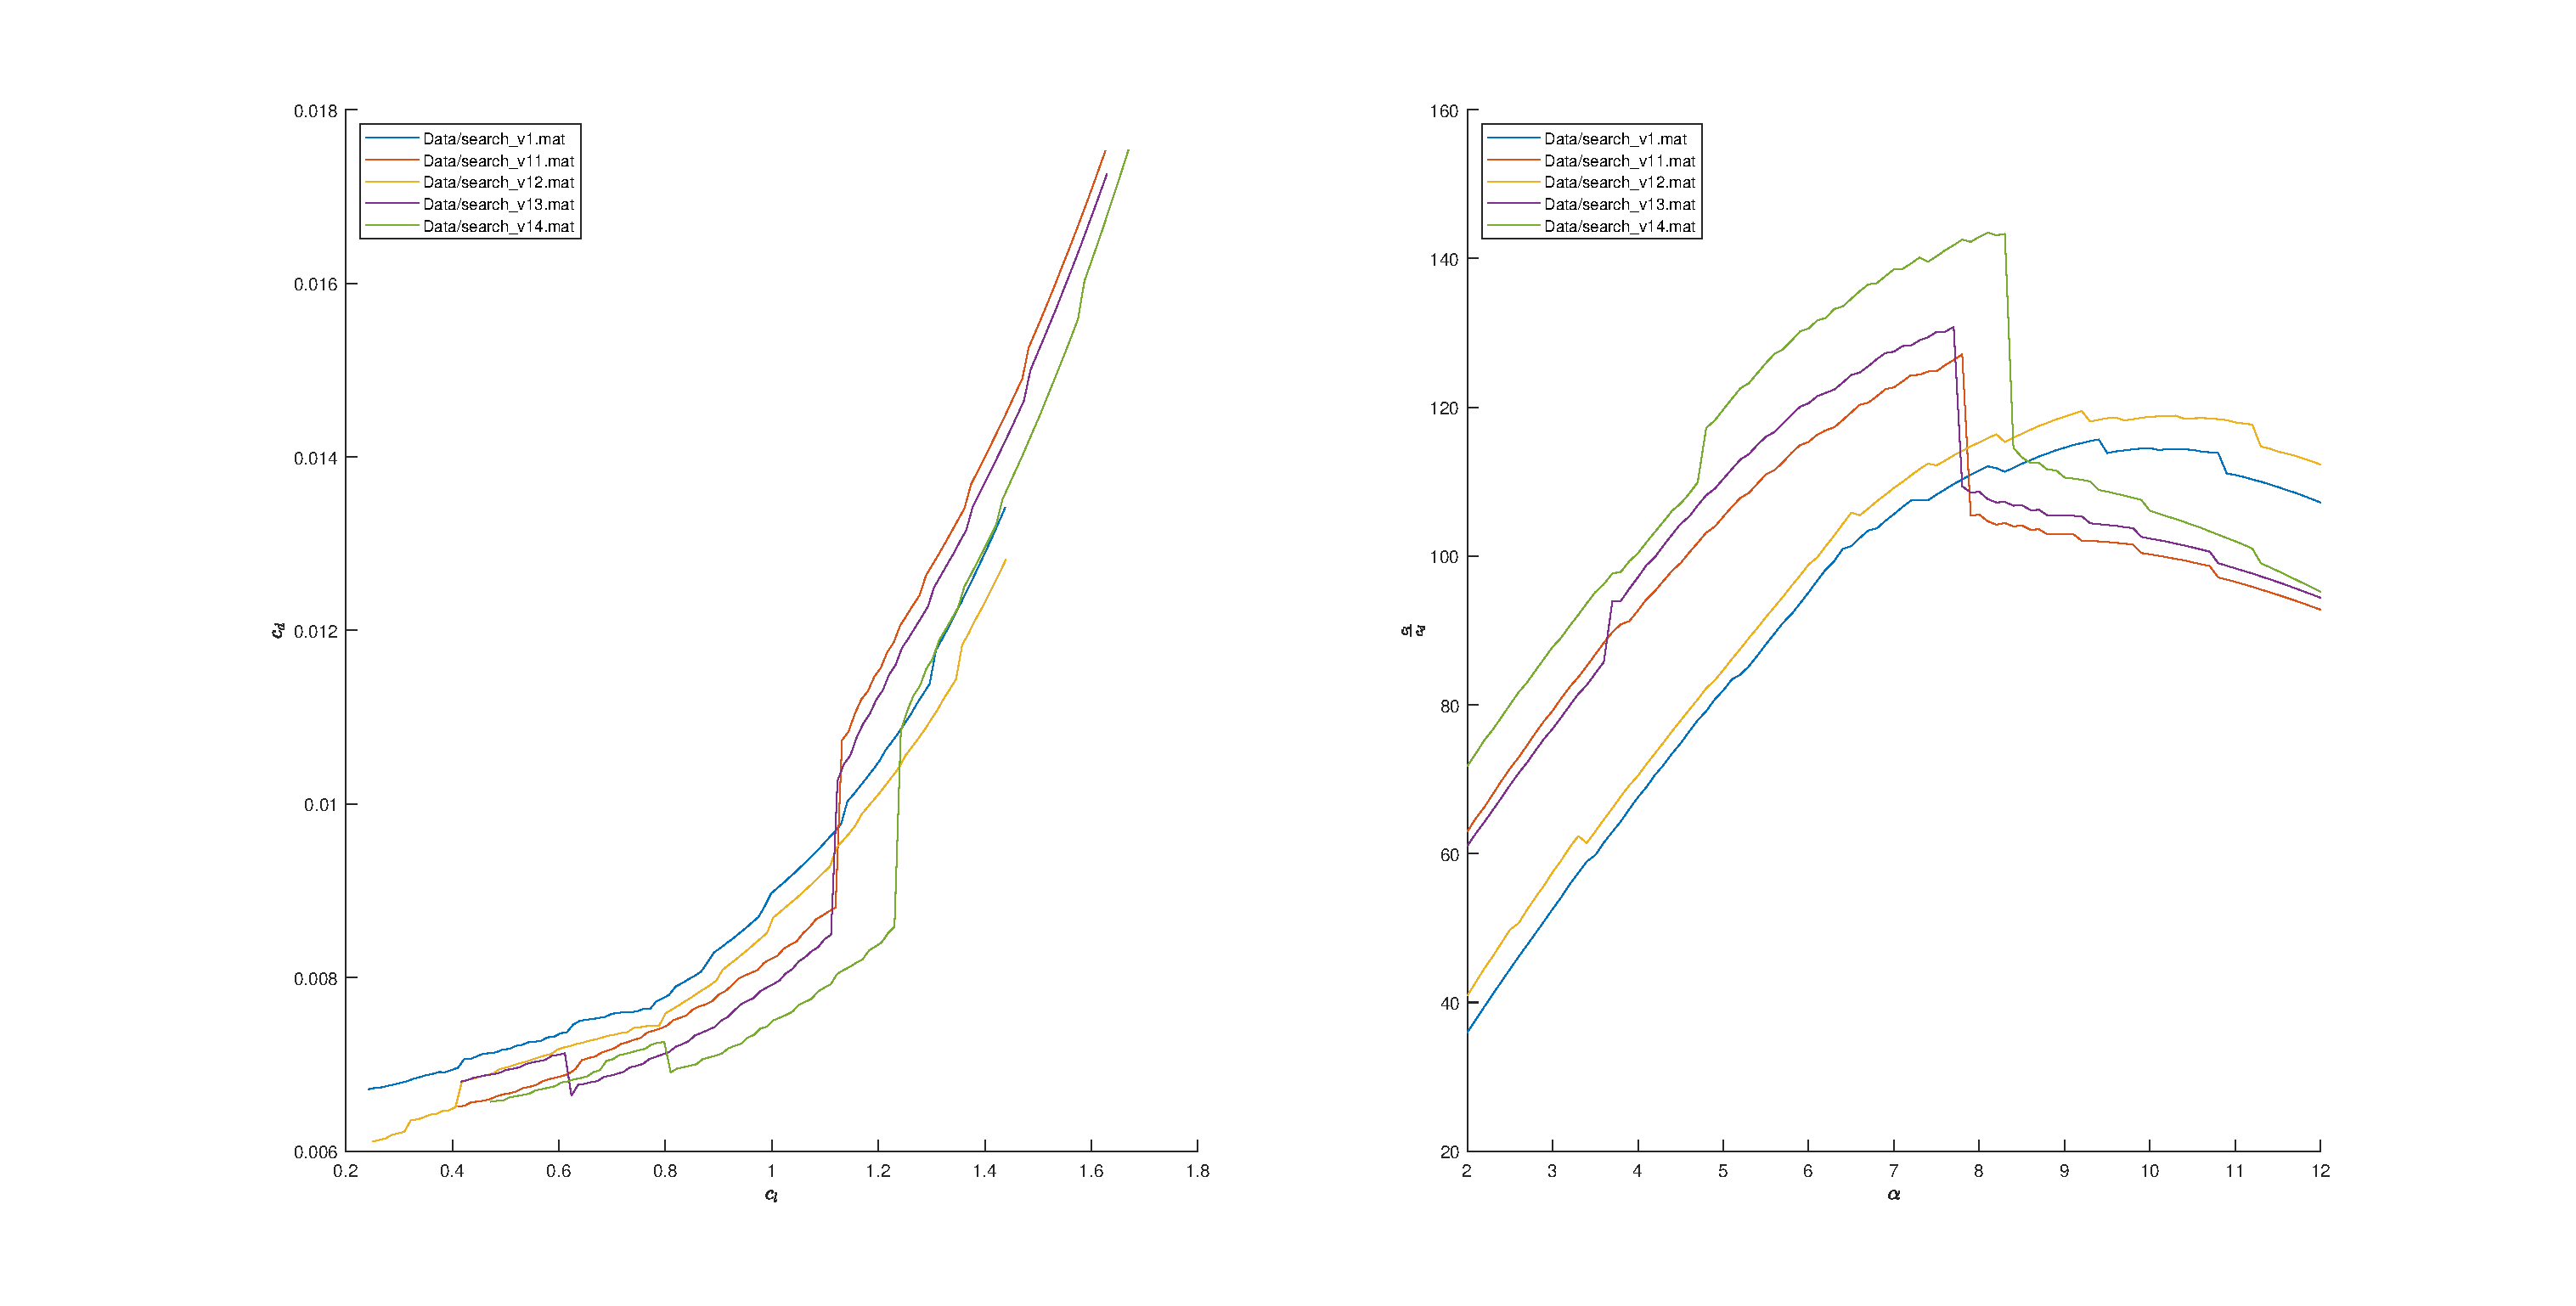
\includegraphics[width=1.2\textwidth, center]{figures/hiRe_lod_14.eps}
        \caption{Drag polar and lift to drag ratio against angle of attack}
        \label{fig:v14_lod}
    \end{subfigure}
    \caption{}
\end{figure}

\begin{figure}[H]
    \begin{subfigure}{0.49\textwidth}
        \centering
        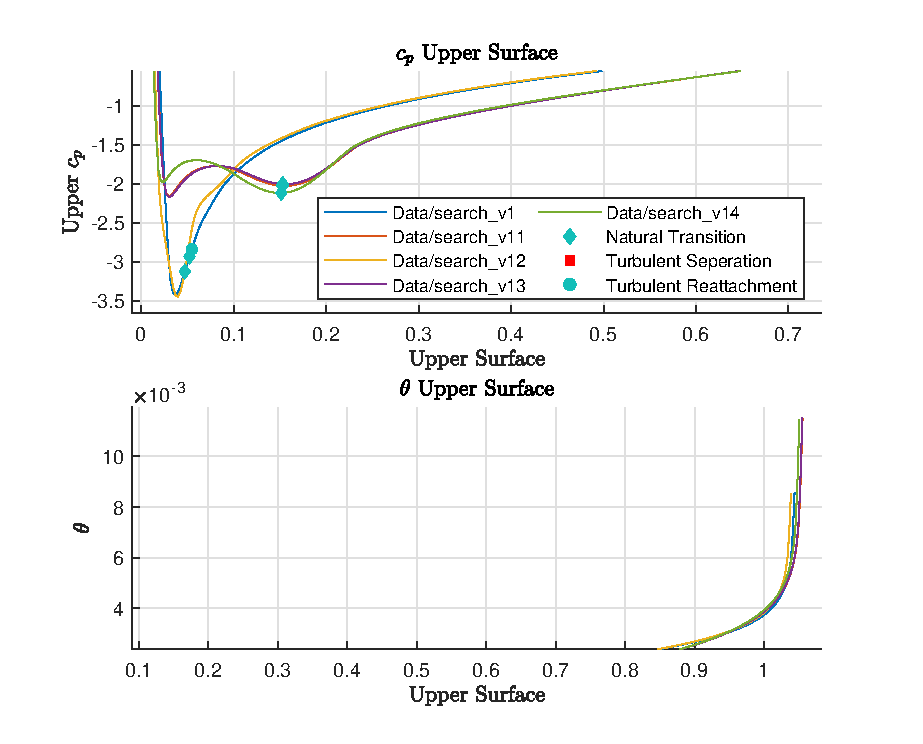
\includegraphics[width=1.1\textwidth, center]{figures/hiRe_upperprofile_14_a7.eps}
        \label{fig:v14_uprofile}
    \end{subfigure}
    \begin{subfigure}{0.49\textwidth}
        \centering
        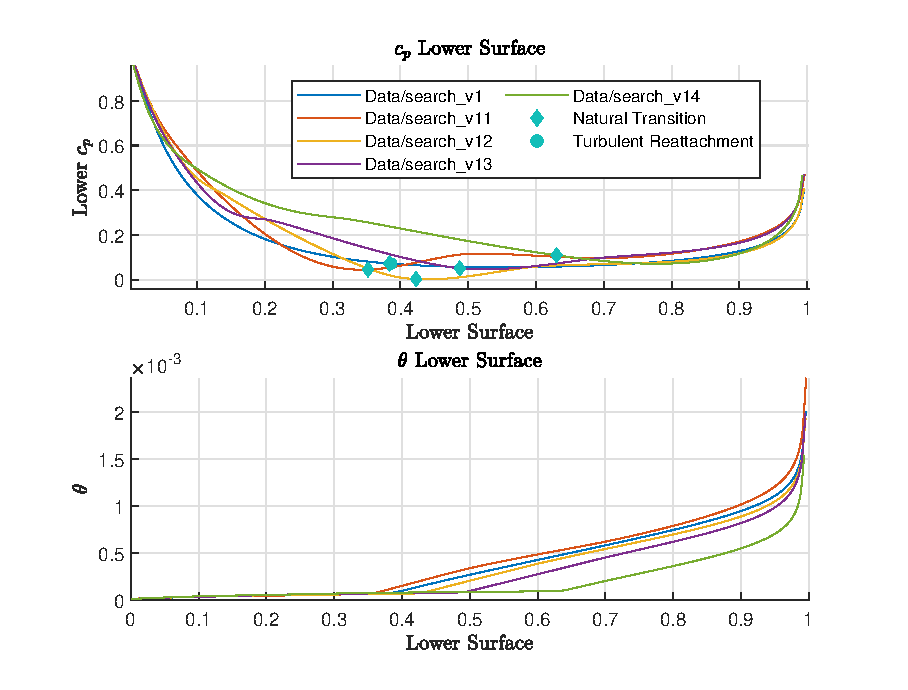
\includegraphics[width=1.15\textwidth, center]{figures/hiRe_lowerprofile_14_a7.eps}
        \label{fig:v14_lprofile}
    \end{subfigure}
    \caption{Upper and lower surface pressure coefficient and momentum thickness profiles for $\alpha = 7^\circ$}
\end{figure}

This improved pressure on the bottom surface and moved transition along which is two desired effects.
Also improved the lift generated on the top surface in a relatively unexpected manner since we didn't change this.
idea moves stagnation point down which increases streamline curvature around top and achieves lower cp on top (more lift)

Changed lower trailing edge to be a tiny bit convex and it was previously concave. 
Approaching concave we get favourable pressure gradient helping to move transition along. 
At concave part we get higher pressures (which for bottom surface increases lift).
Boundary layer turbulent at this point and isn't too badly affected at end. 
Trying to extend concavity further we increased drag as transition occurred earlier. (Approached adverse pressure gradient sooner)


\begin{figure}[H]
    \centering
    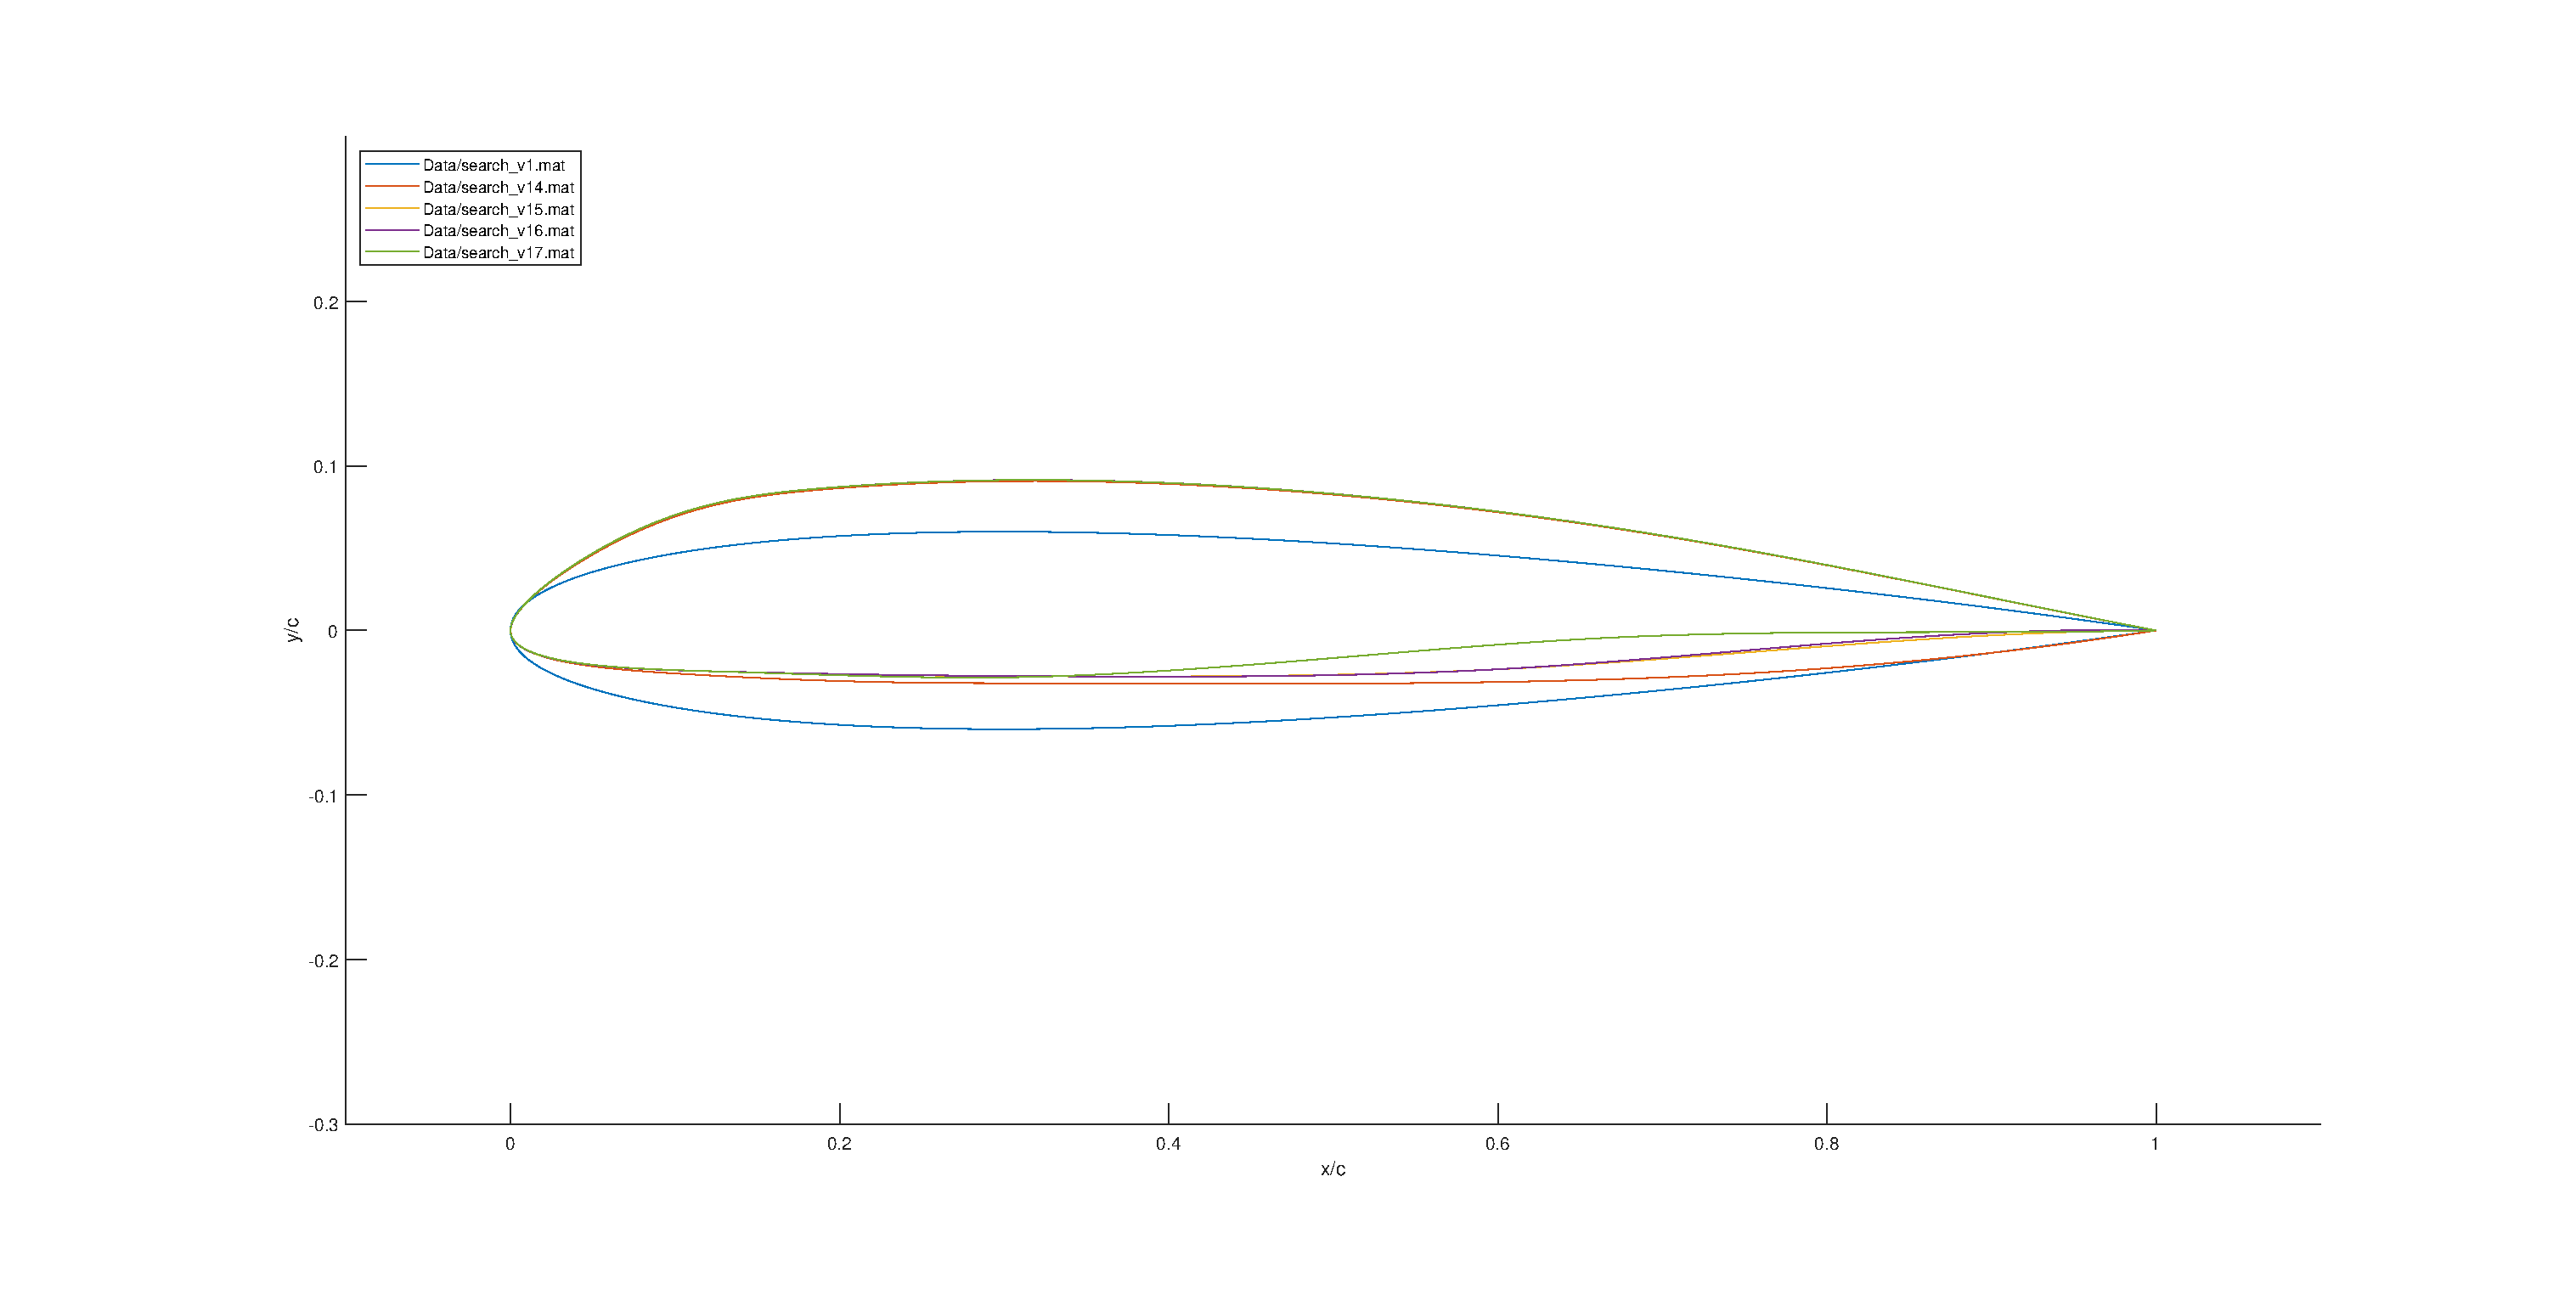
\includegraphics[width=0.8\textwidth]{figures/hiRe_geometry_17.eps}
    \caption{Airfoil}
    \label{fig:v17_geometry}
\end{figure}

\begin{figure}[H]
    \centering
    \begin{subfigure}{0.45\textwidth}
        \centering
        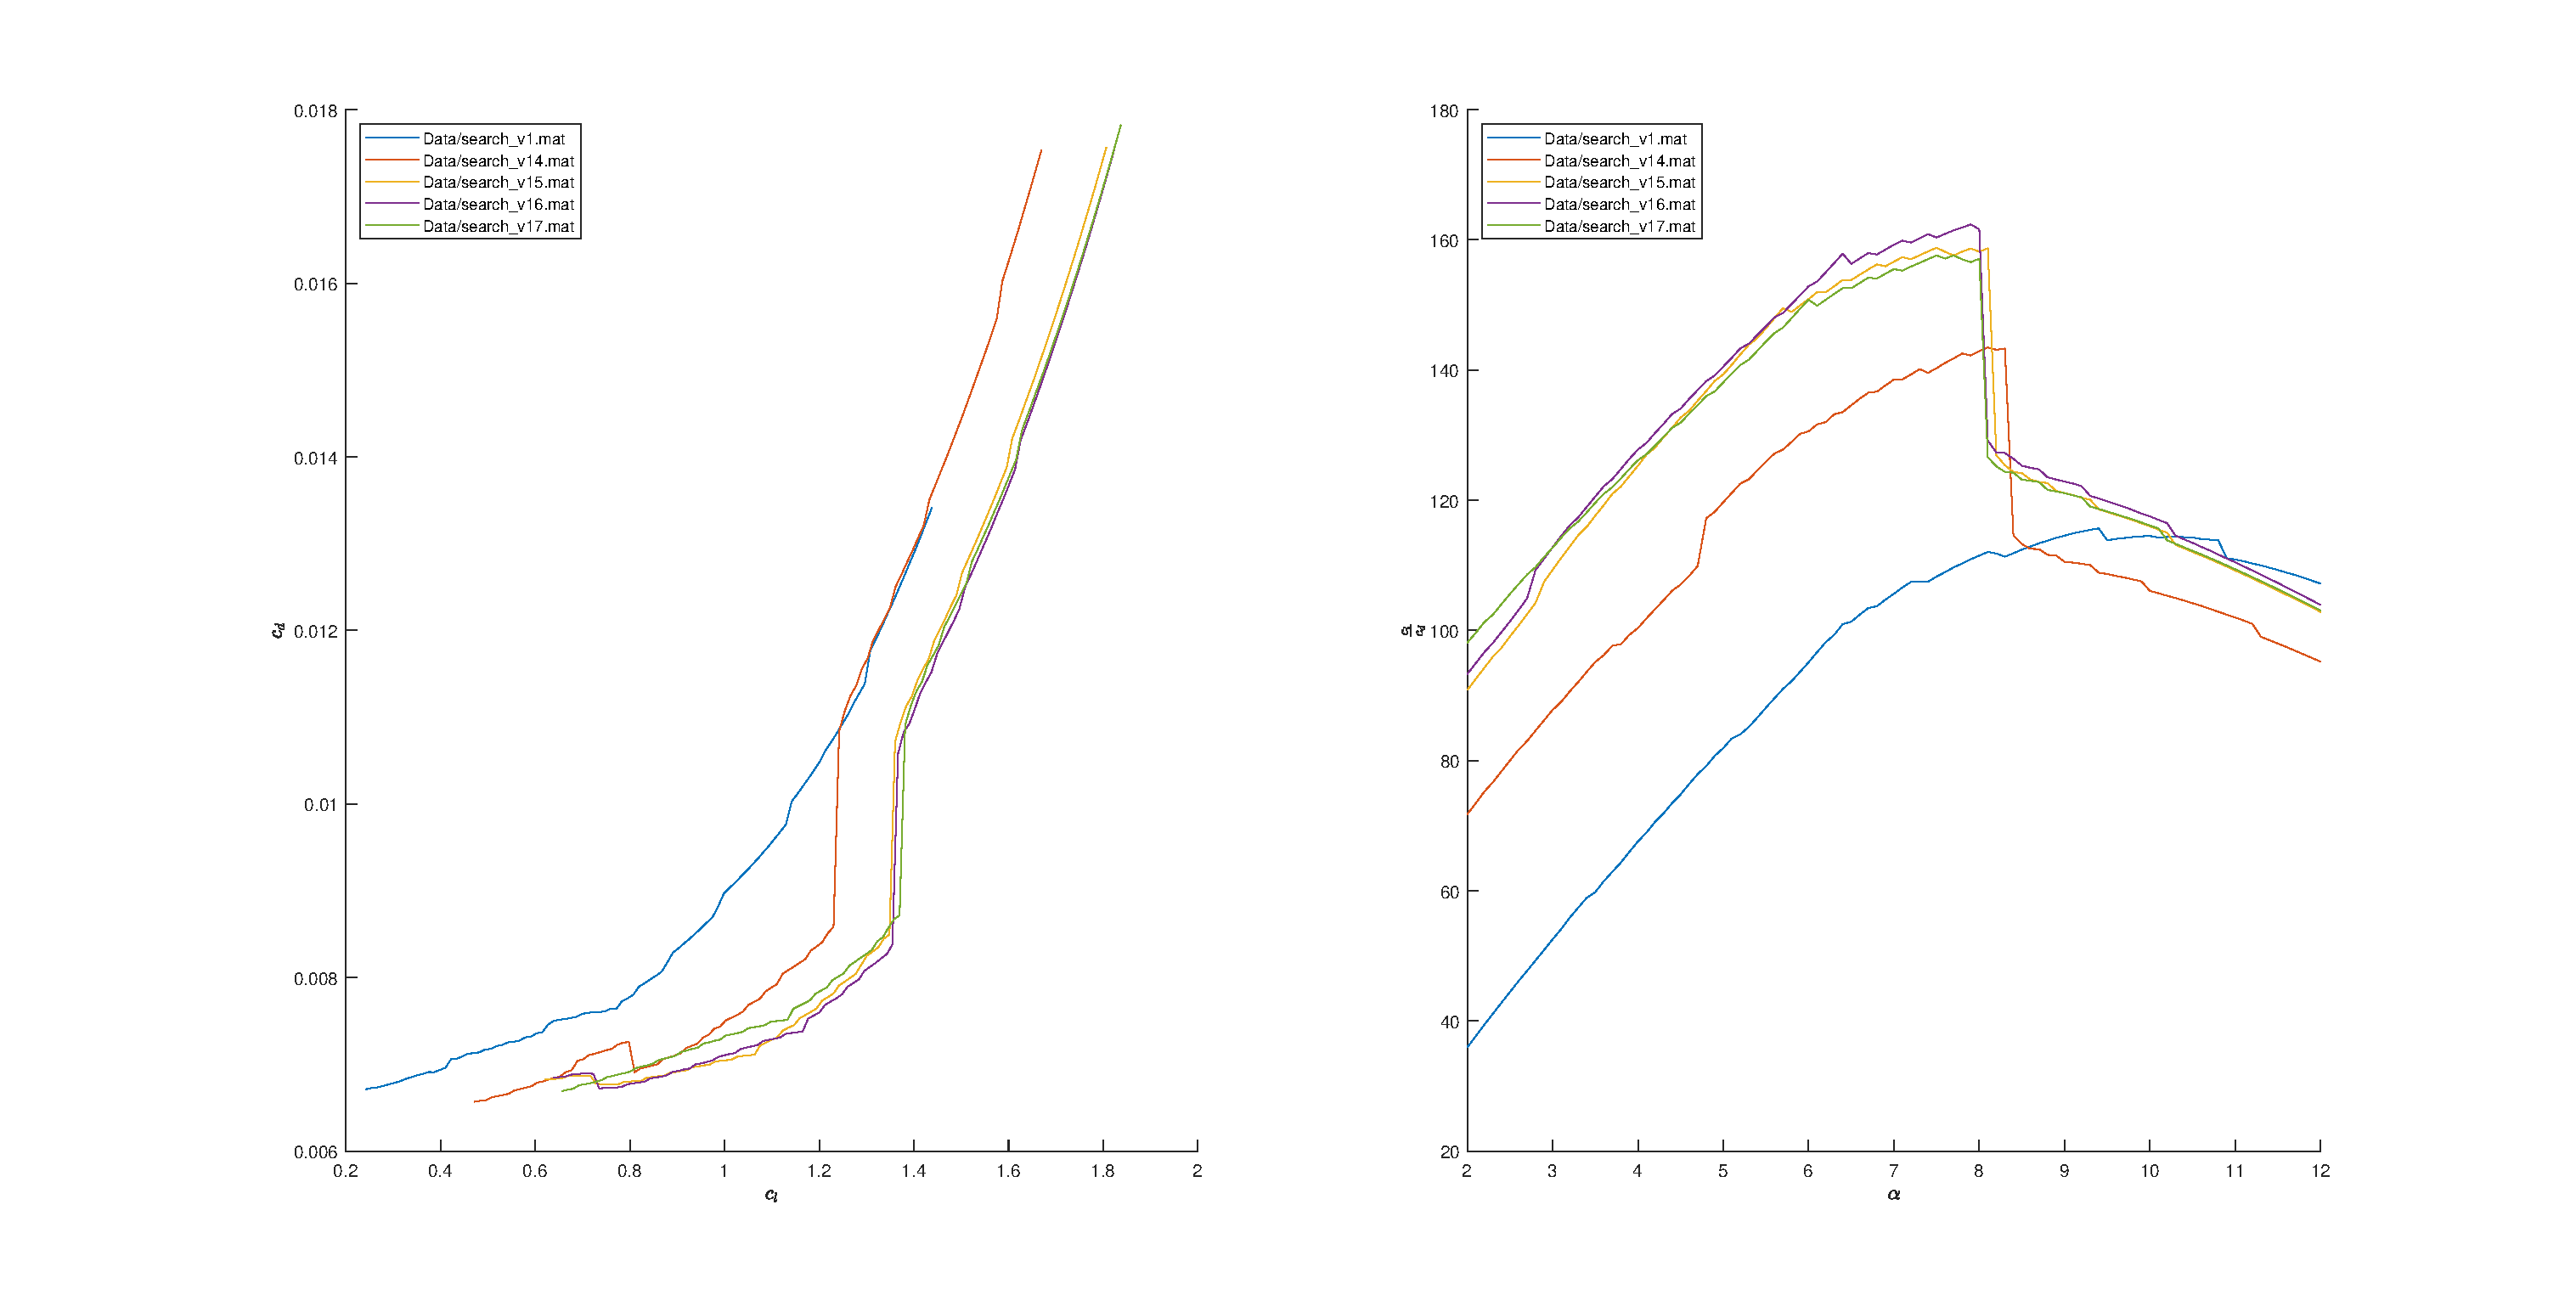
\includegraphics[width=1.2\textwidth, center]{figures/hiRe_lod_17.eps}
        \caption{Airfoil}
        \label{fig:v17_lod}
    \end{subfigure}
    \begin{subfigure}{0.54\textwidth}
        \centering
        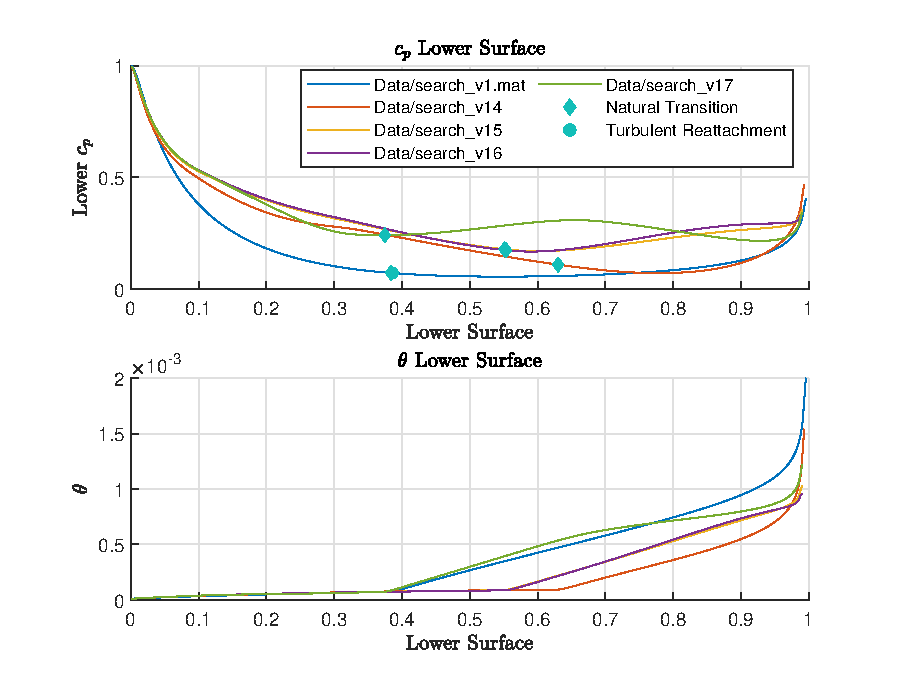
\includegraphics[width=0.99\textwidth]{figures/hiRe_lowerprofile_17_a7.eps}
        \caption{Pressure coefficient and momentum thickness profiles for $\alpha = 7^\circ$}
        \label{fig:v17_lprofile}
    \end{subfigure}
    \caption{Performance of design iterations 14-17 and their upper surface boundary layer profiles}
\end{figure}

Changes to extend the concavity closer to the leading edge saw reductions in drag for V15 and V16.
V17 extended the concavity further but also increased the curvature and introduced a bump with adverse pressure gradient causing early transition and increased drag.
This causes natural transition to occur much later as a favourable pressure gradient was maintained for longer.
The increased curvature also increases pressure coefficient on the lower surface, increasing the lift.

Versions 14 and 16 featured another sudden change in drag, this time a decrease at lower angles of attack.
This was found to be due to a higher stagnation point above the leading edge, which meant that the flow had to turn more sharply around the leading edge.
This caused the boundary layer to transition close to the leading edge and hence the drag to decrease.
This size of the jump was reduced and moved to lower angles of attack by decreasing the curvature of the lower surface near the leading edge.

The best design achieves so far is V16 with a maximum lift to drag ratio of 160.
The next aim was to remove the bump on the lower surface that caused a region of adverse pressure gradient
which caused early transition and increased drag in V17.

\begin{figure}[H]
    \centering
    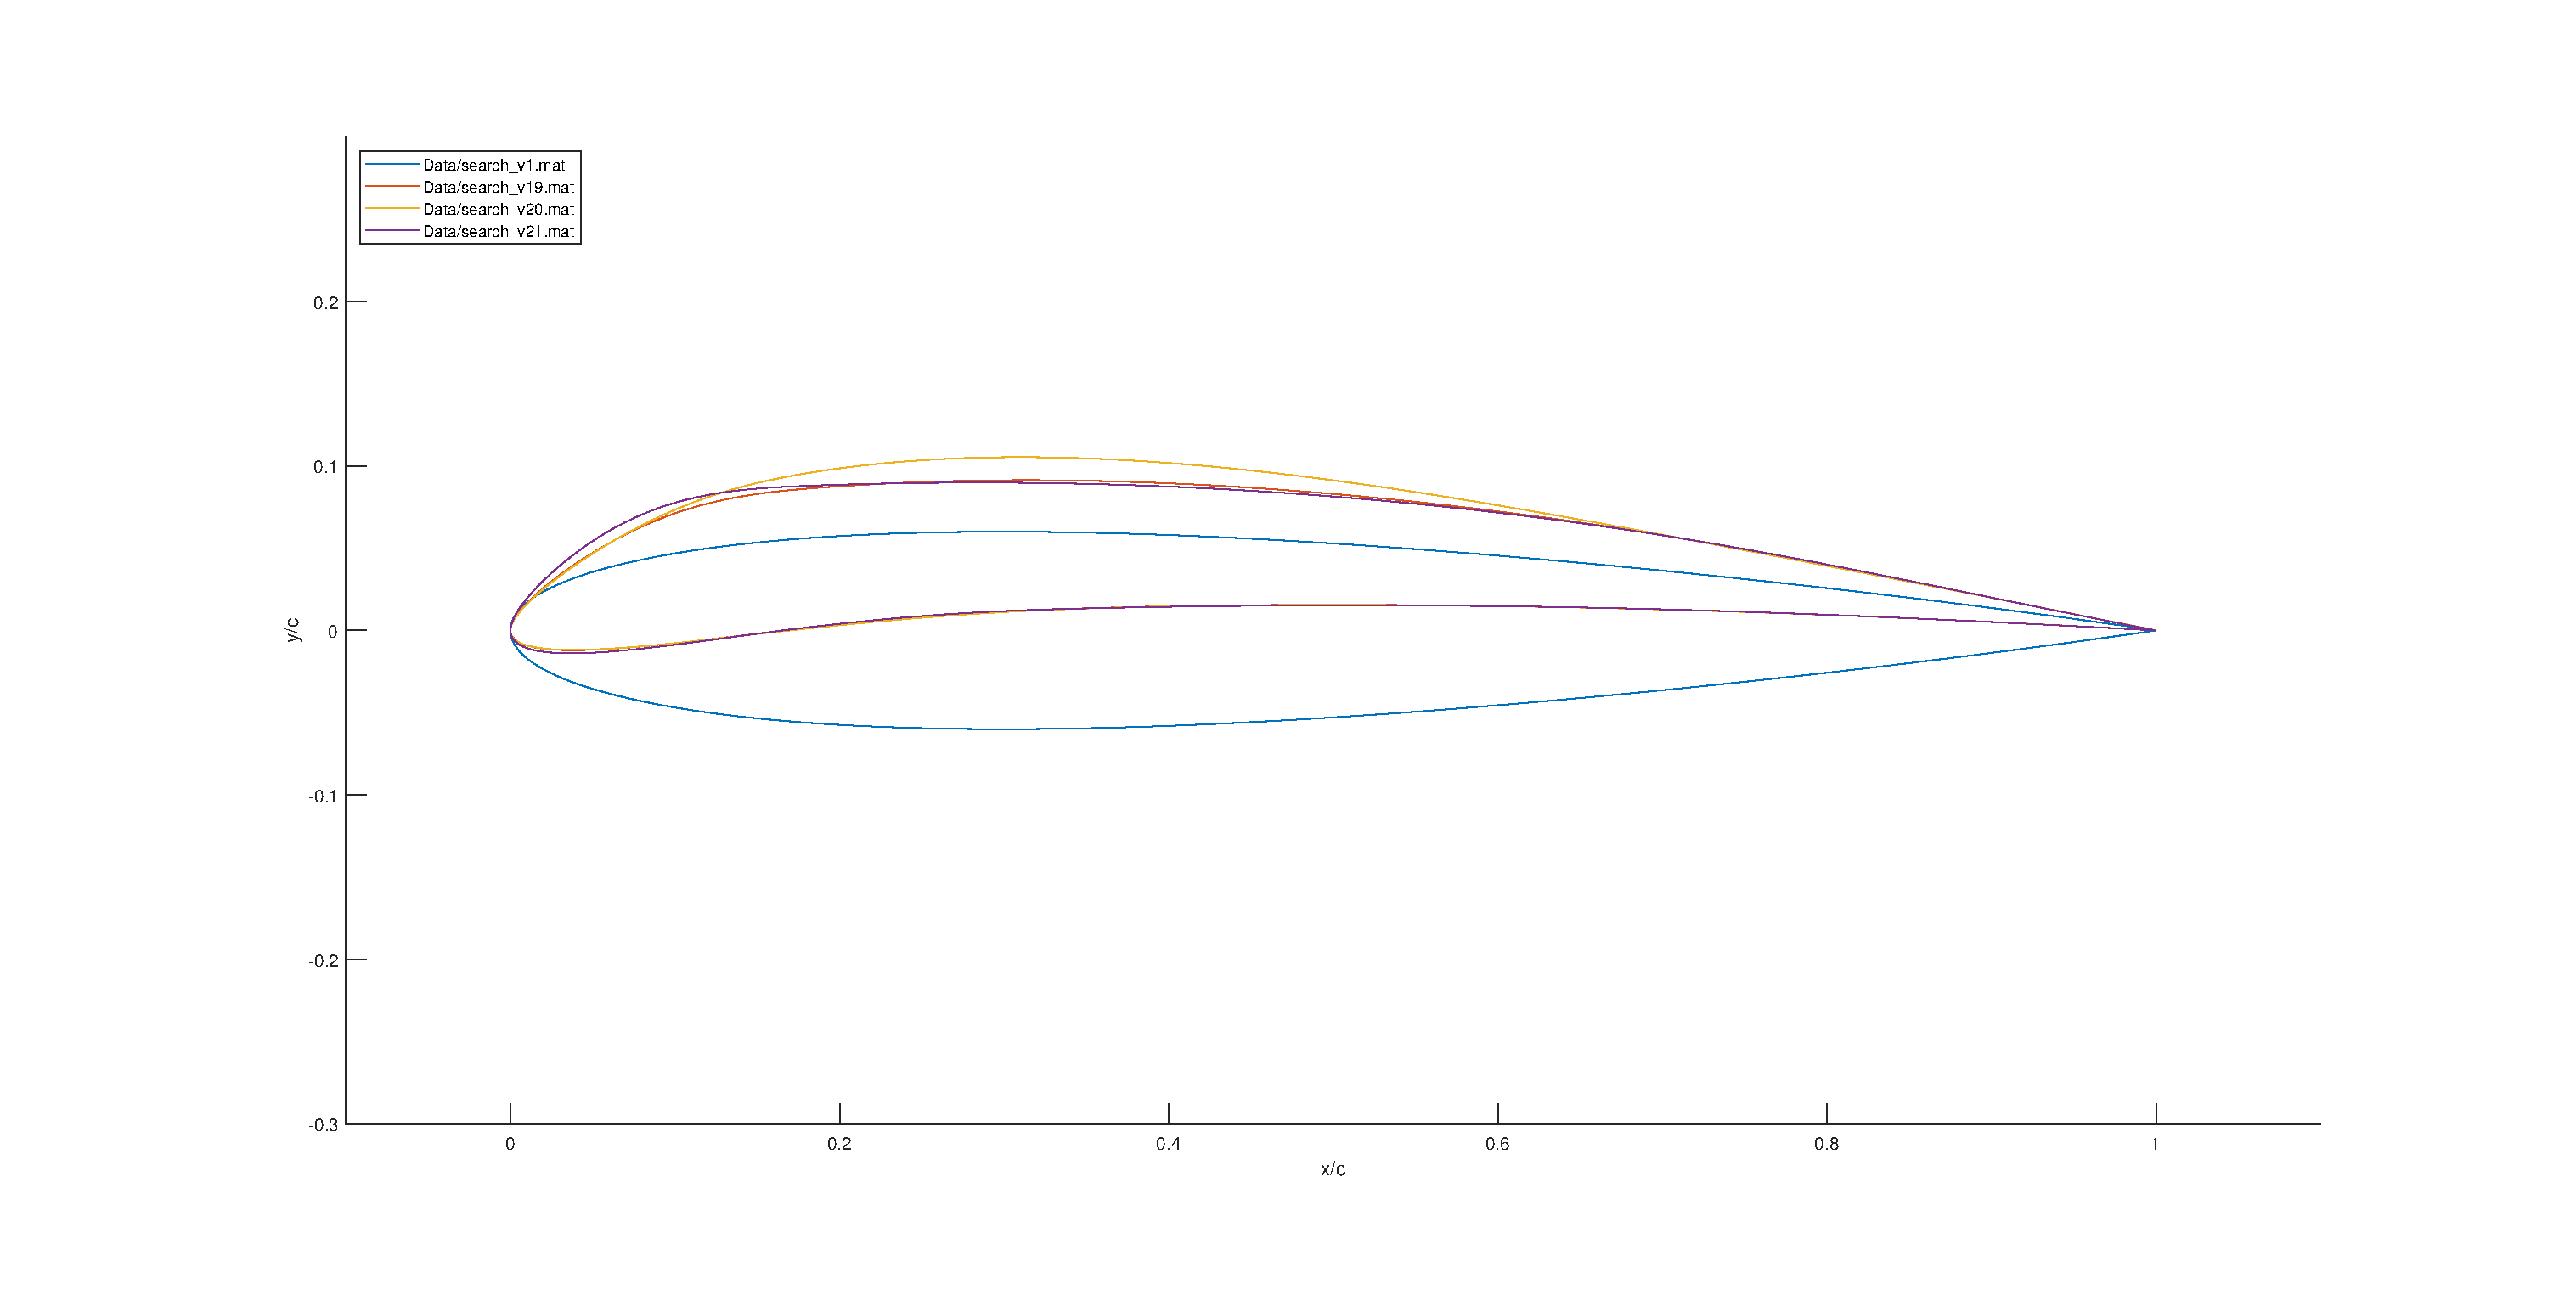
\includegraphics[width=0.8\textwidth]{figures/hiRe_geometry_21.eps}
    \caption{Airfoil}
    \label{fig:v21_geometry}
\end{figure}

\begin{figure}[H]
    \centering
    \begin{subfigure}{0.45\textwidth}
        \centering
        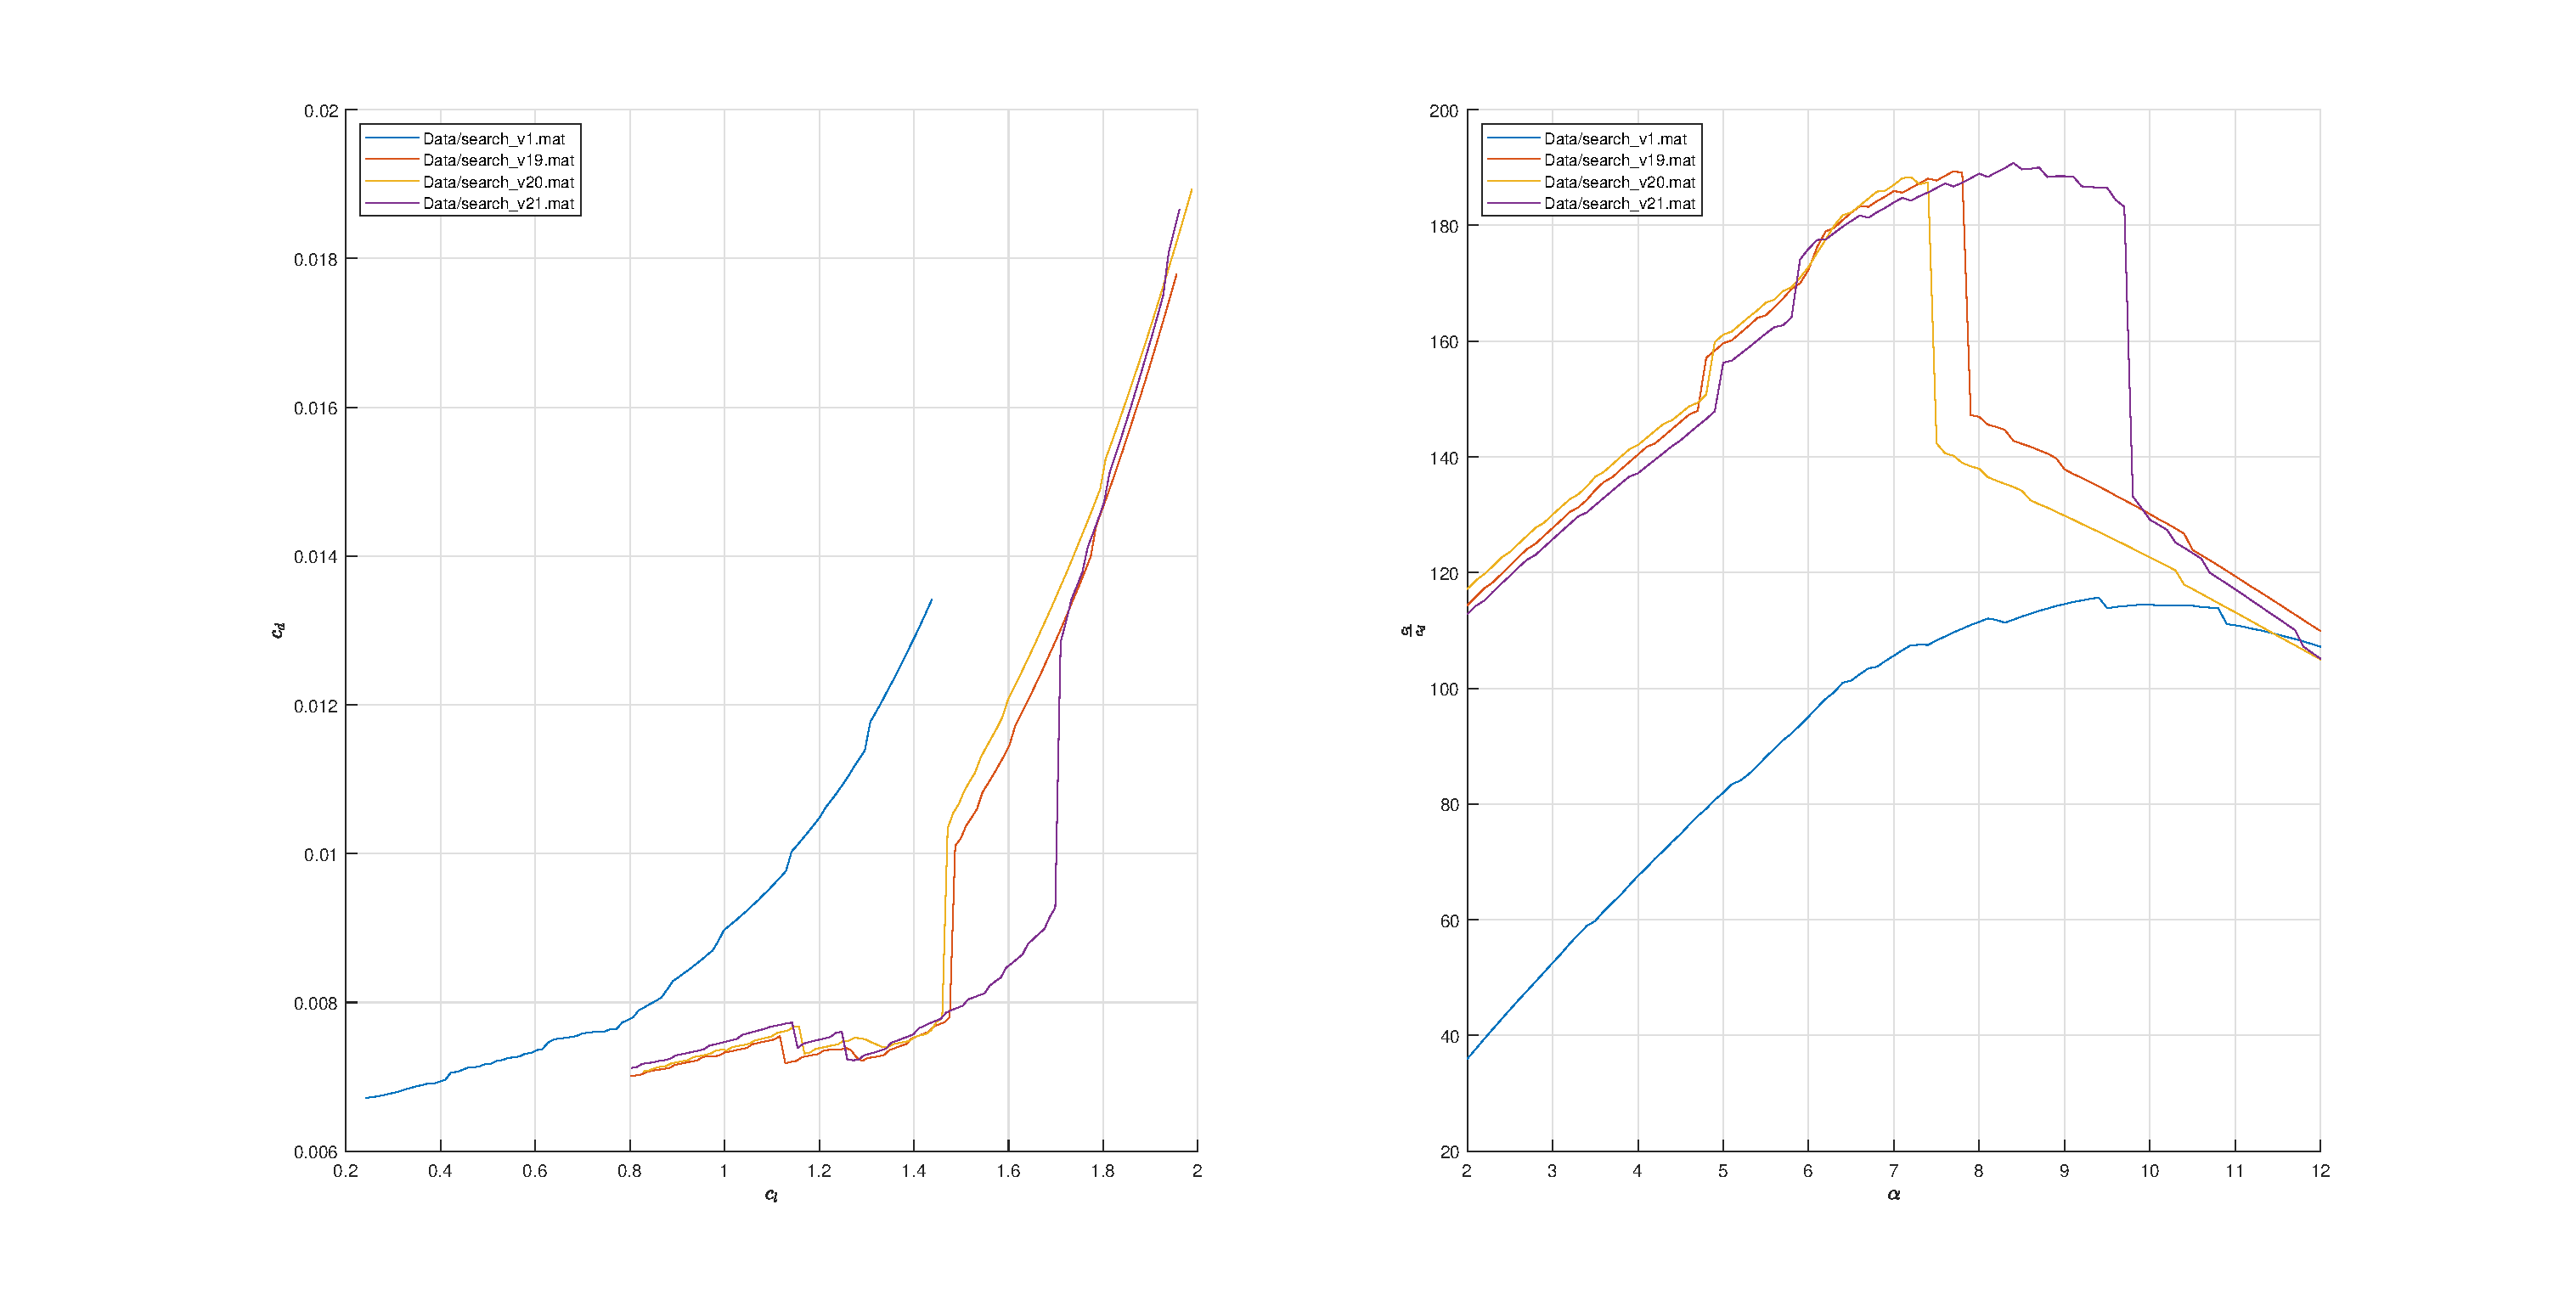
\includegraphics[width=1.2\textwidth, center]{figures/hiRe_lod_21.eps}
        \caption{Airfoil}
        \label{fig:v21_lod}
    \end{subfigure}
    \begin{subfigure}{0.54\textwidth}
        \centering
        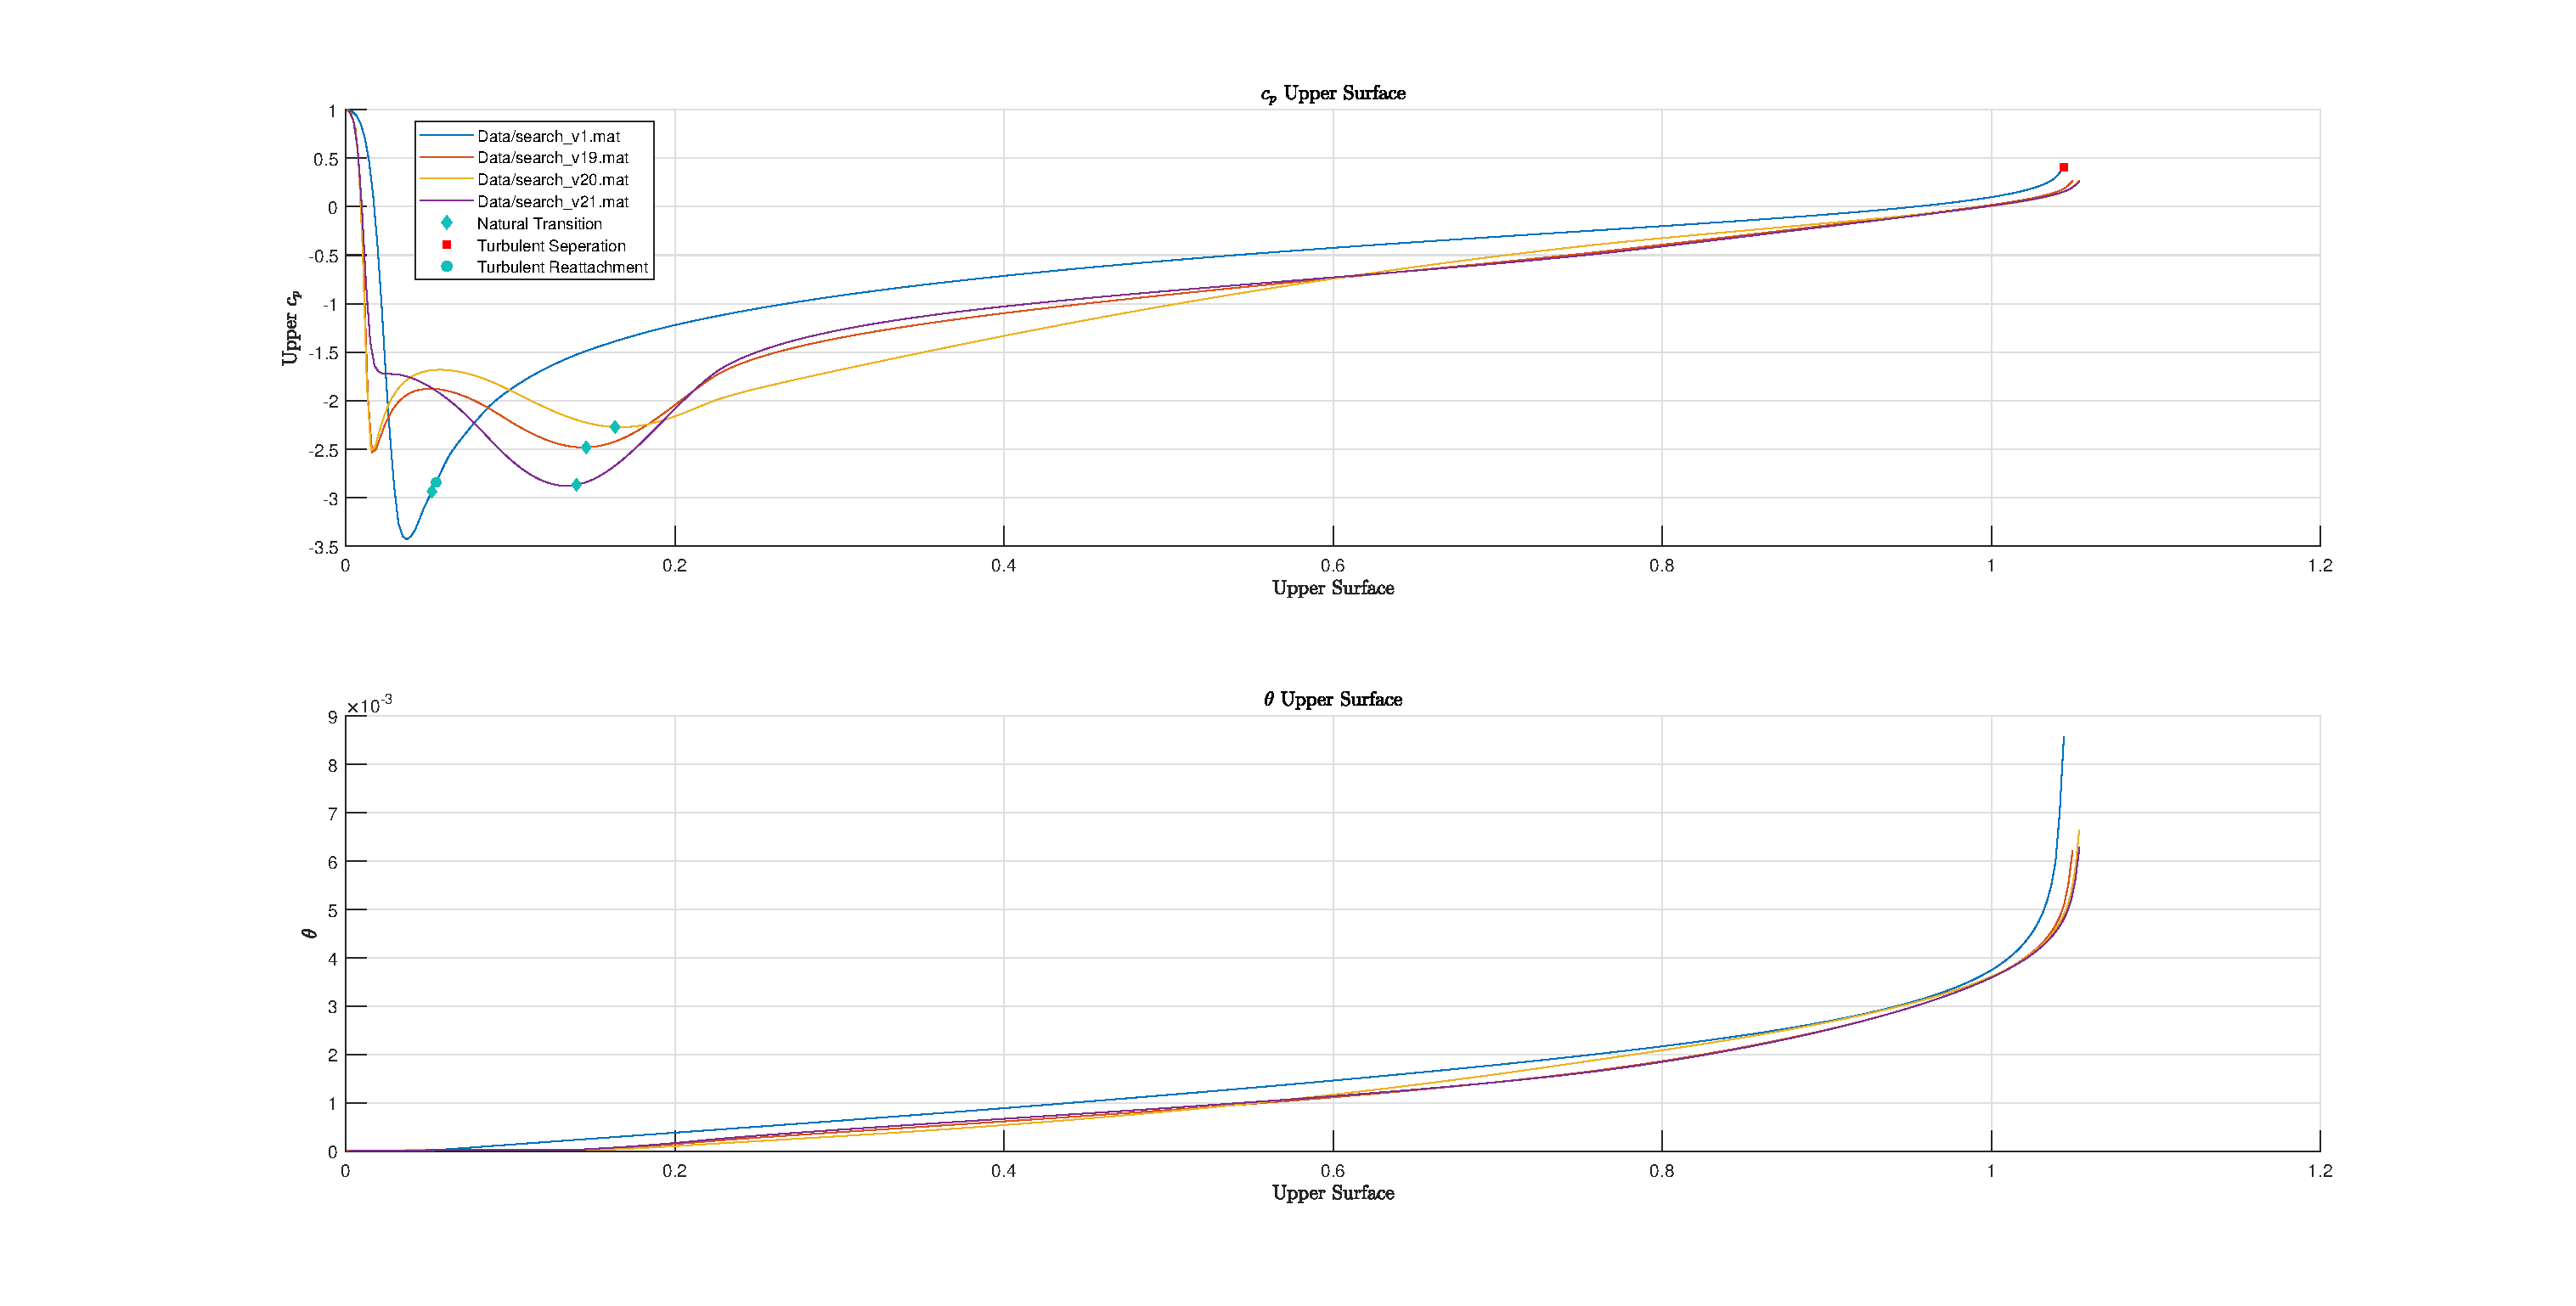
\includegraphics[width=0.99\textwidth]{figures/hiRe_upperprofile_21_a7.eps}
        \caption{Pressure coefficient and momentum thickness profiles for $\alpha = 7^\circ$}
        \label{fig:v21_uprofile}
    \end{subfigure}
    \caption{Performance of design iterations 14-17 and their upper surface boundary layer profiles}
\end{figure}

In V20 design the path length of the top surface increased as we moved it up slightly.
This resulted in increased lift and drag.
The increased length caused the momentum thickness to grow more, increasing drag.
The suction peak widened and gave more area and so produced more lift.

V21. The curvature of the leading edge was increased which means that the flow can turn around with a smaller adverse pressure gradient.
This means higher angle of attacks can be reached, with lower stagnation points before the corner of the leading edge is sharp enough to cause early transition.
This is demonstrated by the jump in drag occurring at higher AoA.


\subsection{Low Reynolds Number}



\begin{figure}[H]
    \begin{subfigure}{0.54\textwidth}
        \centering
        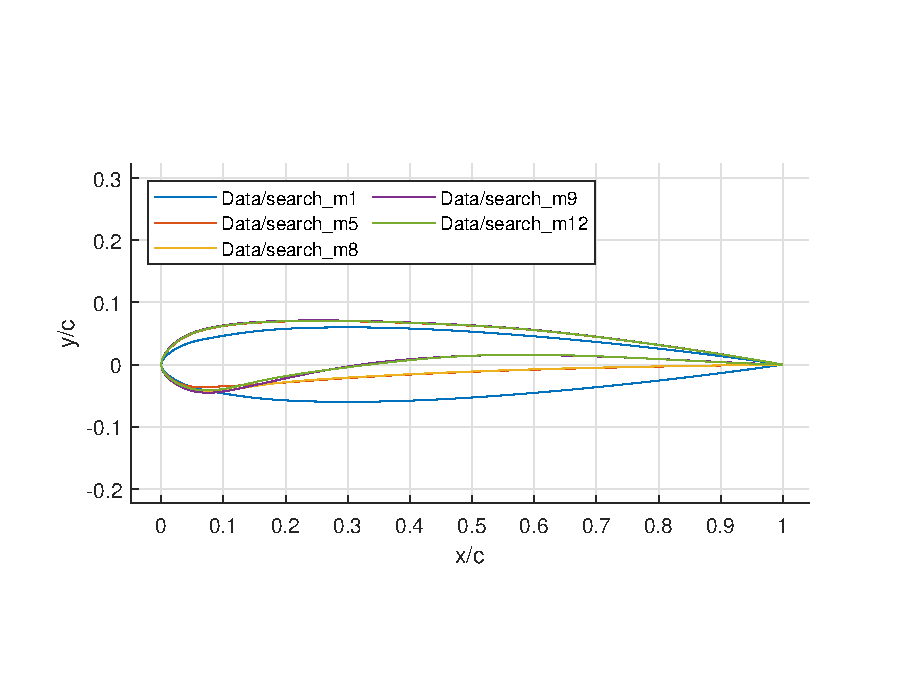
\includegraphics[width=1.2\textwidth, center]{figures/loRe_geometry_12.eps}
        \caption{Airfoil Geometry}
        \label{fig:m12_geometry}
    \end{subfigure}
    \begin{subfigure}{0.45\textwidth}
        \centering
        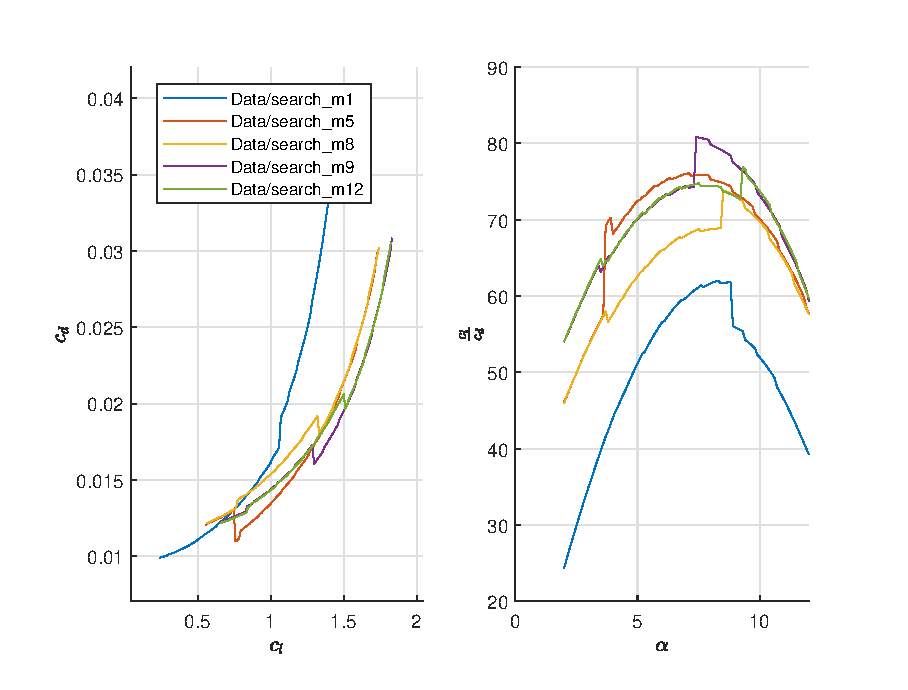
\includegraphics[width=1.2\textwidth, center]{figures/loRe_lod_12.eps}
        \caption{Drag polar and lift to drag ratio against angle of attack}
        \label{fig:m12_lod}
    \end{subfigure}
    \caption{}
\end{figure}

\begin{figure}[H]
    \begin{subfigure}{0.49\textwidth}
        \centering
        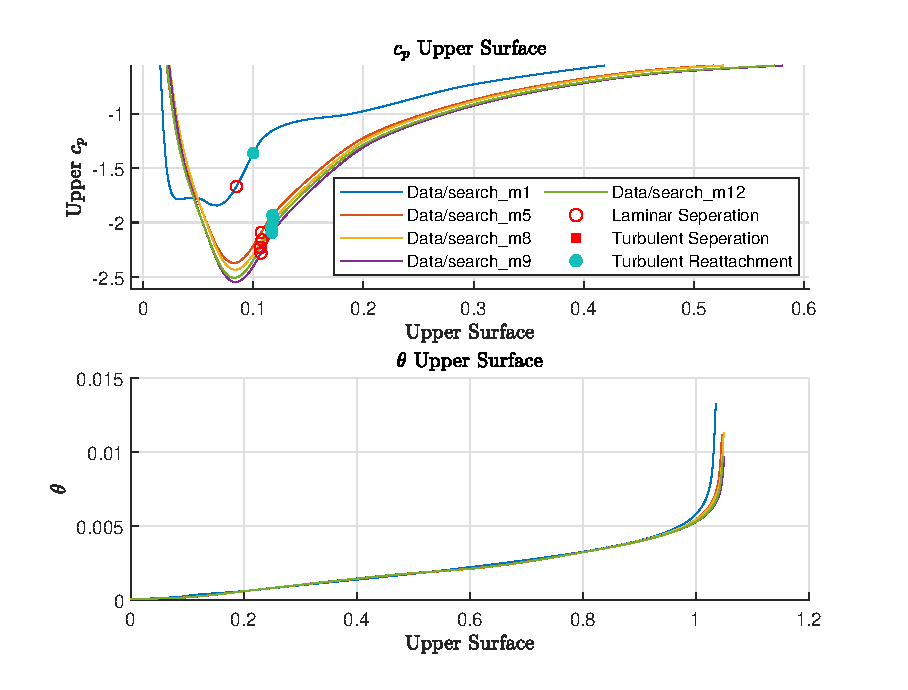
\includegraphics[width=1.1\textwidth, center]{figures/loRe_upperprofile_12_a5.eps}
        \caption{}
        \label{fig:m12_uprofile}
    \end{subfigure}
    \begin{subfigure}{0.49\textwidth}
        \centering
        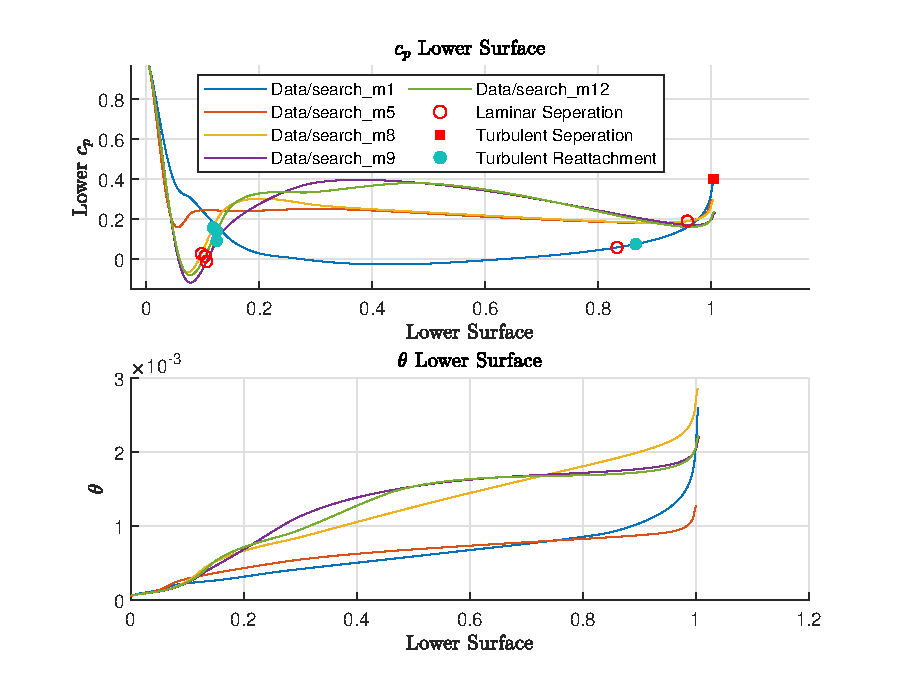
\includegraphics[width=1.15\textwidth, center]{figures/loRe_lowerprofile_12_a5.eps}
        \caption{}
        \label{fig:m12_lprofile}
    \end{subfigure}
    \caption{Upper and lower surface pressure coefficient and momentum thickness profiles for $\alpha = 5^\circ$}
\end{figure}

Laminar seperation and turbulent reattachment was found to occur on the lower surface for initial designs.
Designs with this front seperation bubble forced transition to turbulent flow early instead of laminar seperation at the end.
Seperation at the end of the foil where boundary layer is thicker caused a significant growth in the boundary layer and hence drag.
Additionally forcing the boundary layer to be turbulent means improved tolerance of adverse pressure gradients and so higher pressure coefficients may be reached.
This was exploited in Marks 9 and 12 where the lower surface was made more concave to increase lift at the cost of increased drag.

An attempt was made to move the seperation bubble further back by decreasing the curvature of the bump and adverse pressure gradient behind the bump.

\begin{figure}[H]
    \begin{subfigure}{0.54\textwidth}
        \centering
        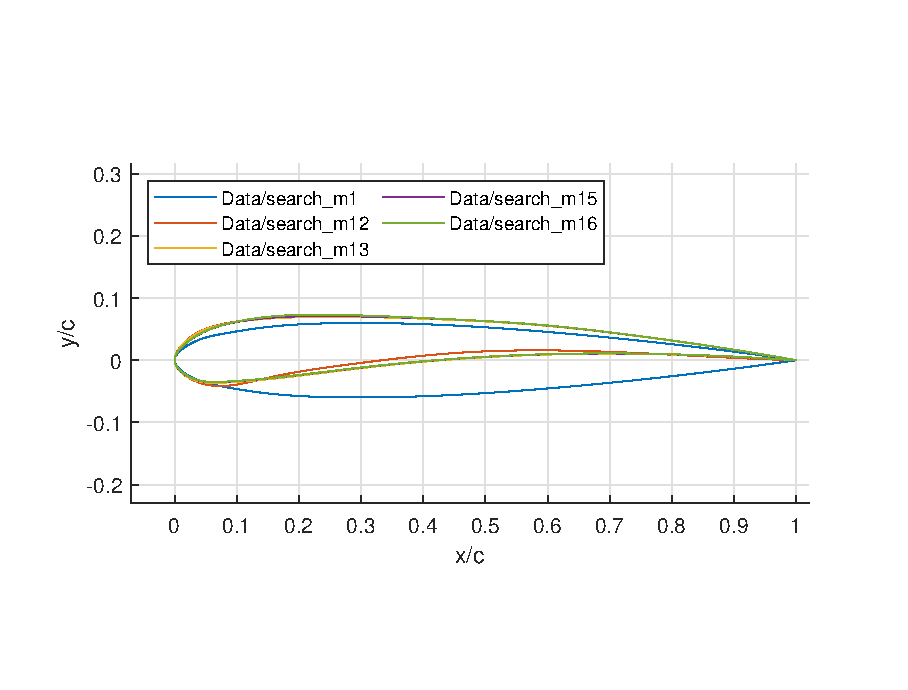
\includegraphics[width=1.2\textwidth, center]{figures/loRe_geometry_16.eps}
        \caption{Airfoil Geometry}
        \label{fig:m16_geometry}
    \end{subfigure}
    \begin{subfigure}{0.45\textwidth}
        \centering
        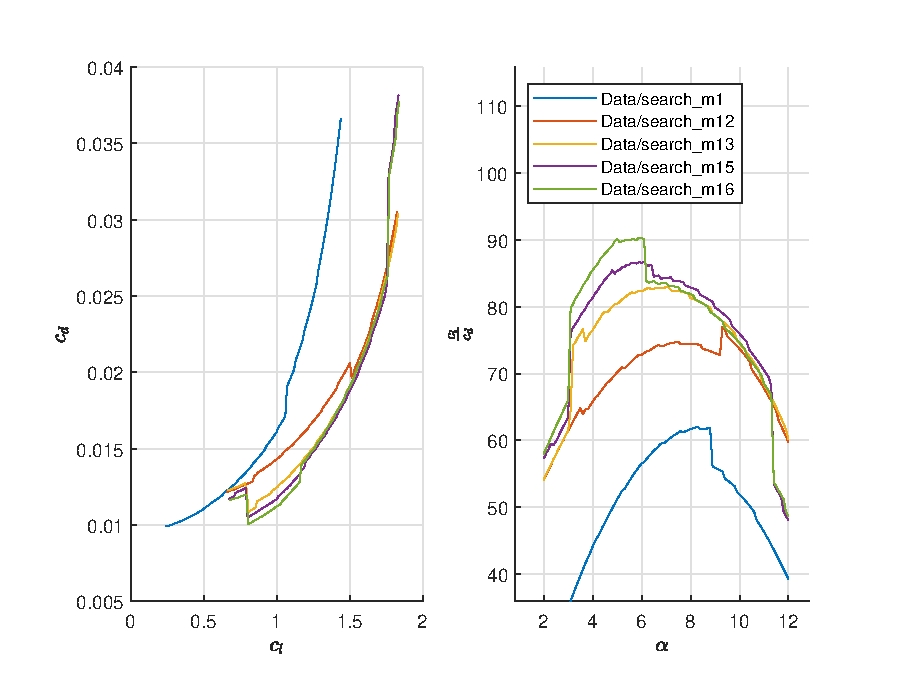
\includegraphics[width=1.2\textwidth, center]{figures/loRe_lod_16.eps}
        \caption{Drag polar and lift to drag ratio against angle of attack}
        \label{fig:m16_lod}
    \end{subfigure}
    \caption{}
\end{figure}

\begin{figure}[H]
    \begin{subfigure}{0.49\textwidth}
        \centering
        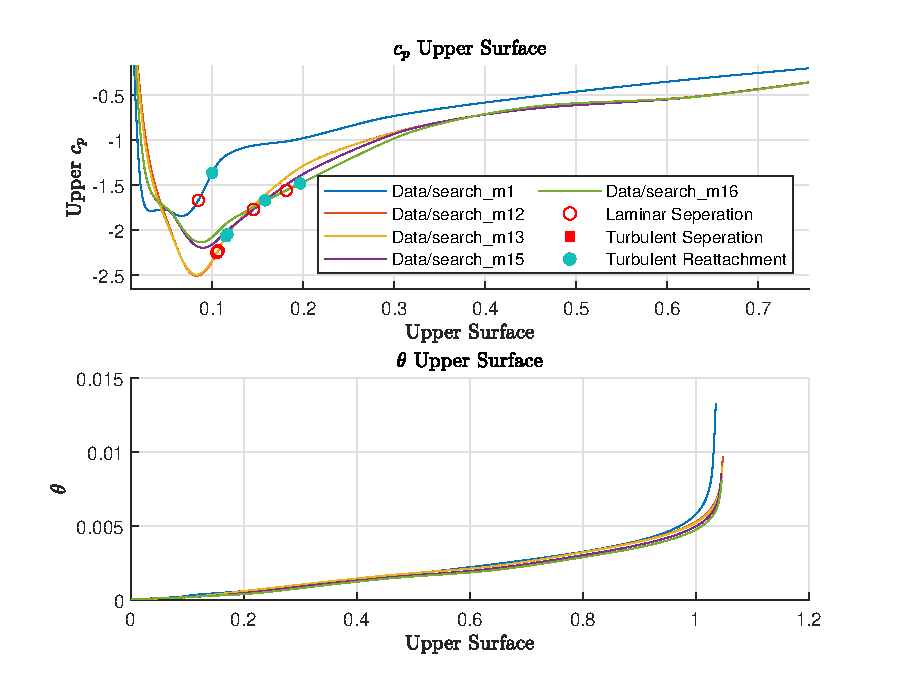
\includegraphics[width=1.1\textwidth, center]{figures/loRe_upperprofile_16_a5.eps}
        \caption{}
        \label{fig:m16_uprofile}
    \end{subfigure}
    \begin{subfigure}{0.49\textwidth}
        \centering
        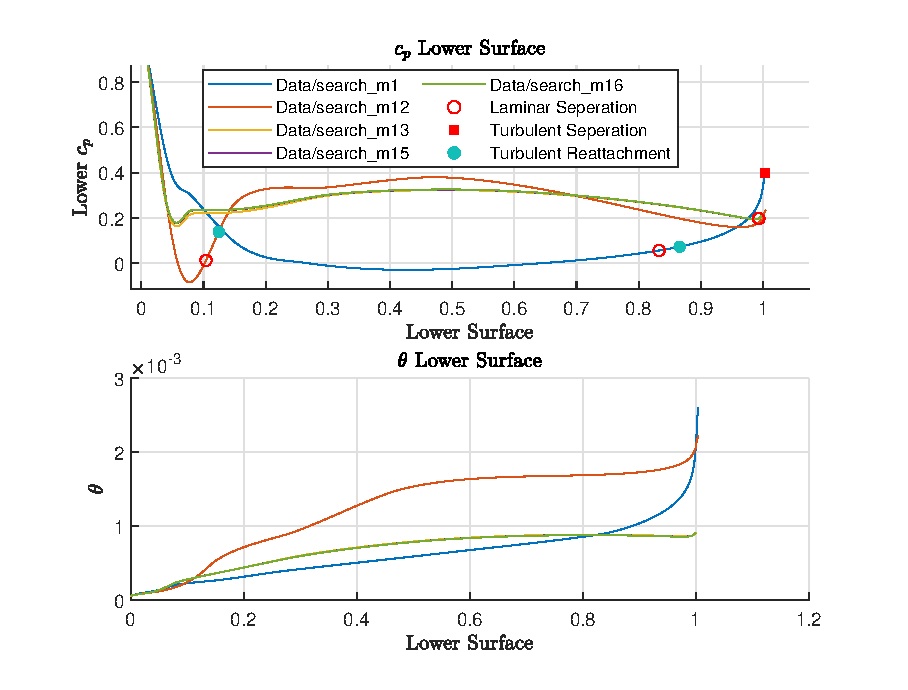
\includegraphics[width=1.15\textwidth, center]{figures/loRe_lowerprofile_16_a5.eps}
        \caption{}
        \label{fig:m16_lprofile}
    \end{subfigure}
    \caption{Upper and lower surface pressure coefficient and momentum thickness profiles for $\alpha = 5^\circ$}
\end{figure}

The lift slightly increased and the drag significantly decreased.
This removed the front seperation bubble, similar to Mark 5 of figure \ref{fig:m12_lprofile} with separation occuring near trailing edge.
However the drag was much lower than Mark 5 due to reduced adverse pressure gradient from reduced curvature at the trailing edge.
This was found to significantly increase the lift to drag ratio suggesting that the bubble, although it gave better performance than the original NACA0012, was not an optimal aerofoil.

Changes made to marks 13, 15 and 16 were done to push the seperation bubble further back and reduce the adverse pressure gradients to reduce drag.
This involved increasing radius of curvature of the bump and 
were shaped to be even thicker aerofoils to achieve a larger curve radius which successfully pushed back the separation bubble, at the cost of increased length for boundary layer growth.
These changes were found to be very sensitive and so it may not be possible to push the upper surface separation point as far back as the lower surface.

\begin{figure}[H]
    \centering
    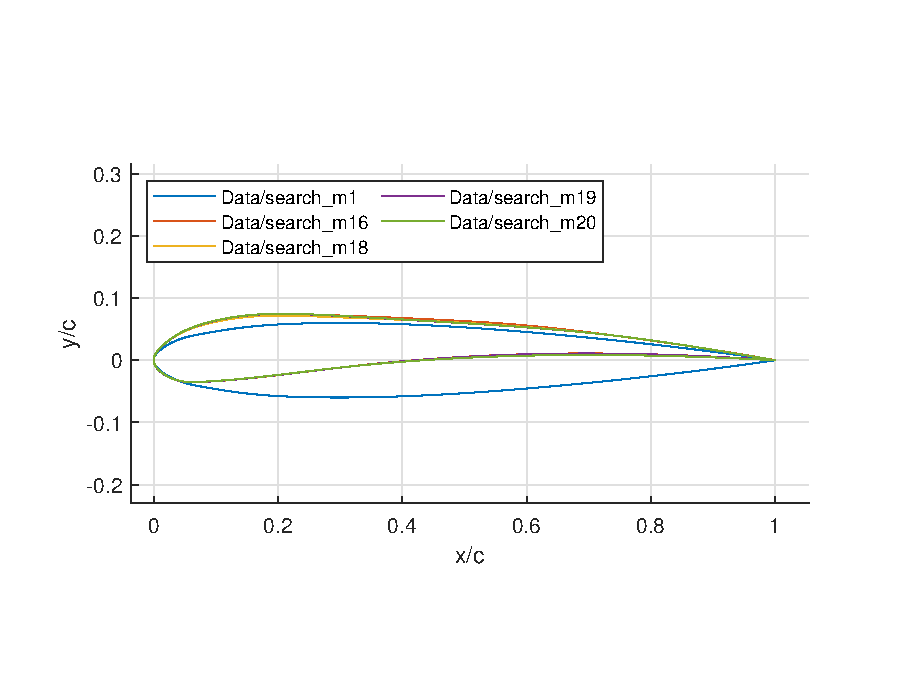
\includegraphics[width=0.8\textwidth]{figures/loRe_geometry_20.eps}
    \caption{Airfoil}
    \label{fig:m20_geometry}
\end{figure}

\begin{figure}[H]
    \begin{subfigure}{0.49\textwidth}
        \centering
        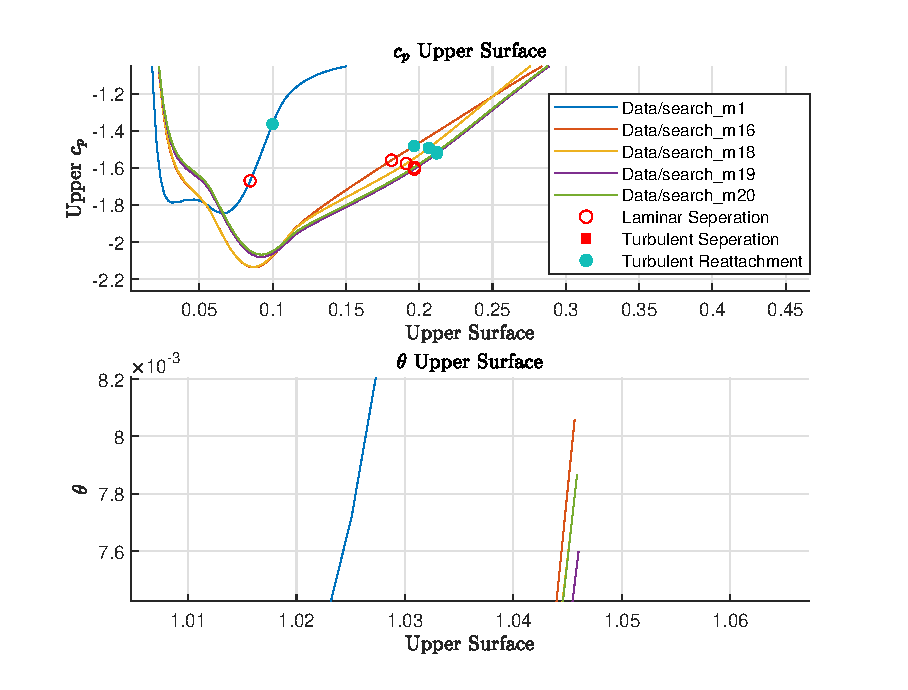
\includegraphics[width=1.1\textwidth, center]{figures/loRe_upperprofile_20_a5.eps}
        \caption{}
        \label{fig:m20_uprofile}
    \end{subfigure}
    \begin{subfigure}{0.49\textwidth}
        \centering
        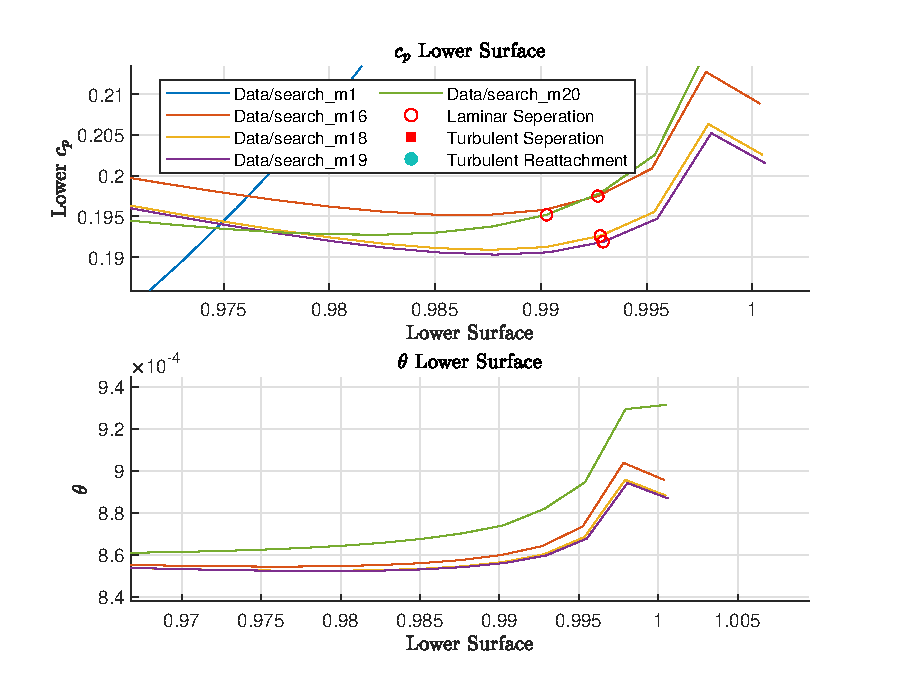
\includegraphics[width=1.1\textwidth, center]{figures/loRe_lowerprofile_20_a5.eps}
        \caption{}
        \label{fig:m20_lprofile}
    \end{subfigure}
    \caption{Upper and lower surface pressure coefficient and momentum thickness profiles for $\alpha = 5^\circ$}
\end{figure}

Design marks 18 and 19 were shaped to be even thicker aerofoils to achieve a larger curve radius which successfully pushed back the separation bubble, at the cost of increased length for boundary layer growth.
This still provided a marginal improvement in drag but not enough to be further considered.

Mark 20 had reduced lower surface curvature close to the trailing edge in attempt to reduce the adverse pressure gradient and move seperation point further back.
This change only increased the gradient upstream and so resulted in loss of lift and increased drag.

Focus was then placed on moving the upper surface seperation bubble further back to reduce drag.
This was done by smoothing the top surface to decrease pressure gradients.


\begin{figure}[H]
    \centering
    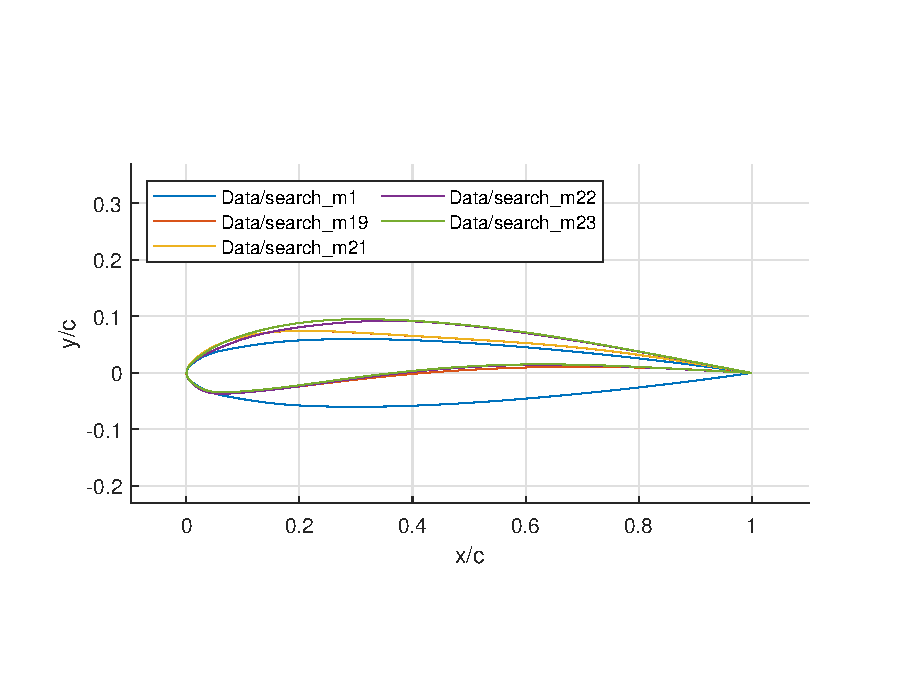
\includegraphics[width=0.8\textwidth]{figures/loRe_geometry_23.eps}
    \caption{Airfoil}
    \label{fig:m23_geometry}
\end{figure}

\begin{figure}[H]
    \centering
    \begin{subfigure}{0.45\textwidth}
        \centering
        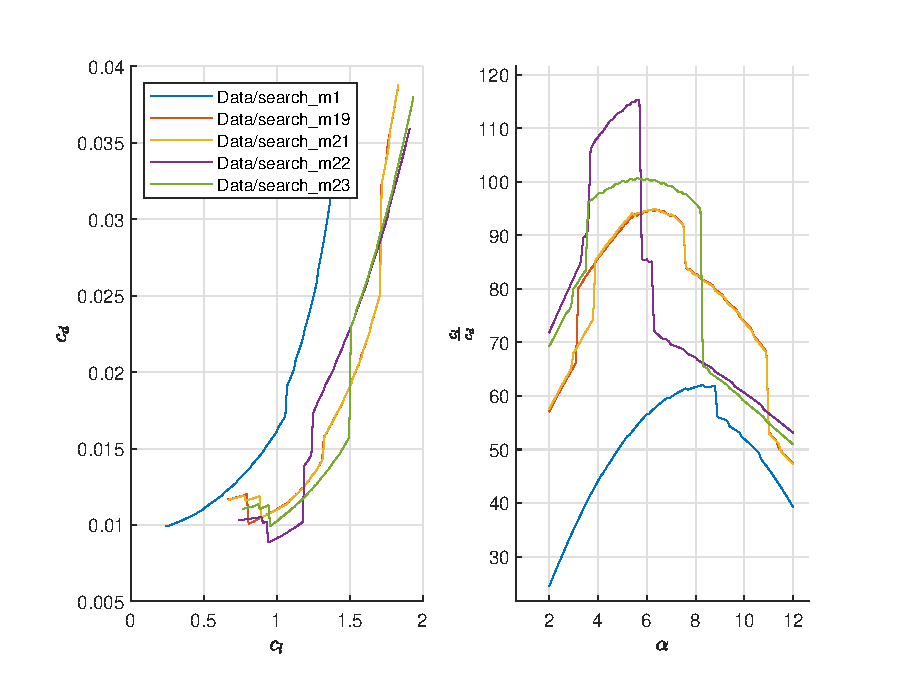
\includegraphics[width=1.2\textwidth, center]{figures/loRe_lod_23.eps}
        \caption{Airfoil}
        \label{fig:m23_lod}
    \end{subfigure}
    \begin{subfigure}{0.54\textwidth}
        \centering
        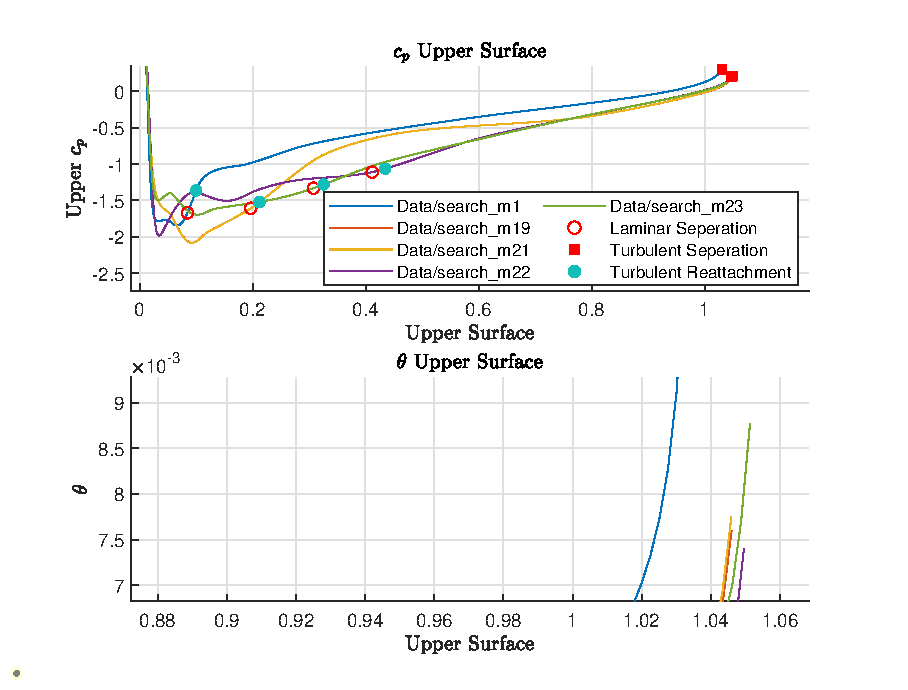
\includegraphics[width=0.99\textwidth]{figures/loRe_upperprofile_23_a5.eps}
        \caption{Pressure coefficient and momentum thickness profiles for $\alpha = 7^\circ$}
        \label{fig:m23_uprofile}
    \end{subfigure}
    \caption{Performance of design iterations 21-23 and their upper surface boundary layer profiles}
\end{figure}



These changes showed a improvement over mark 21 still there but transition occurring on adverse p grad slightly earlier. 

Marks 24 and 25 consisted of more aggressive changes which ended up creating a suction at the start which performs poorly.

An attempt to fix this was made by continuing the curvature further. 

\begin{figure}[H]
    \centering
    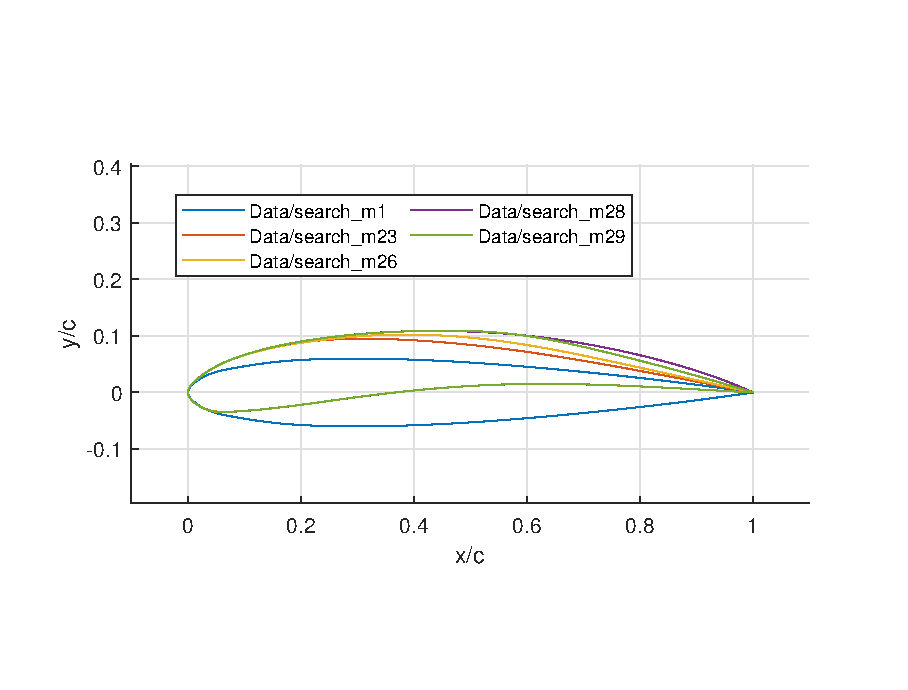
\includegraphics[width=0.8\textwidth]{figures/loRe_geometry_29.eps}
    \caption{Airfoil}
    \label{fig:m29_geometry}
\end{figure}

\begin{figure}[H]
    \centering
    \begin{subfigure}{0.45\textwidth}
        \centering
        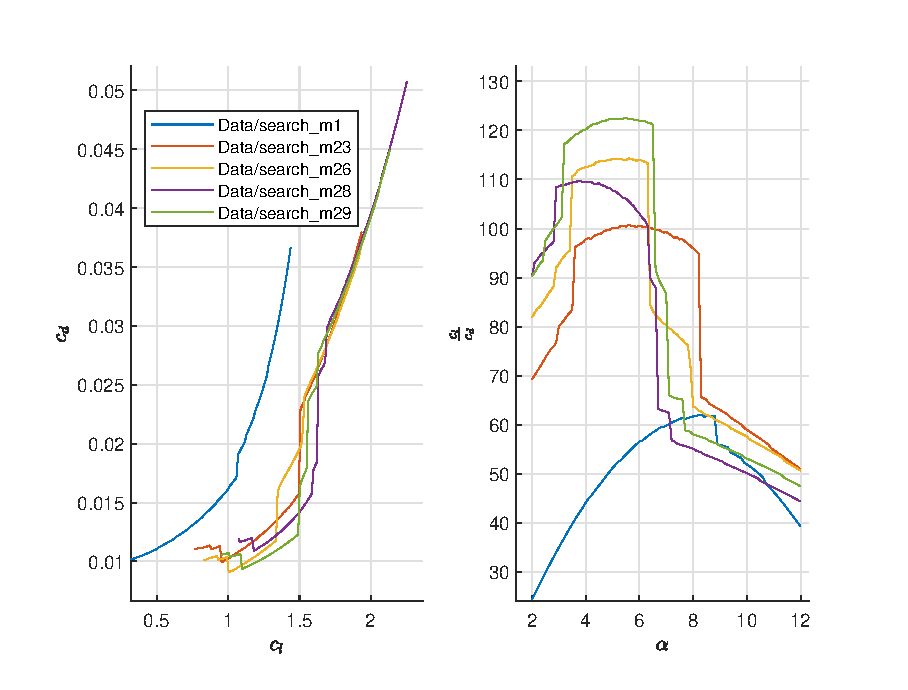
\includegraphics[width=1.2\textwidth, center]{figures/loRe_lod_29.eps}
        \caption{Airfoil}
        \label{fig:m29_lod}
    \end{subfigure}
    \begin{subfigure}{0.54\textwidth}
        \centering
        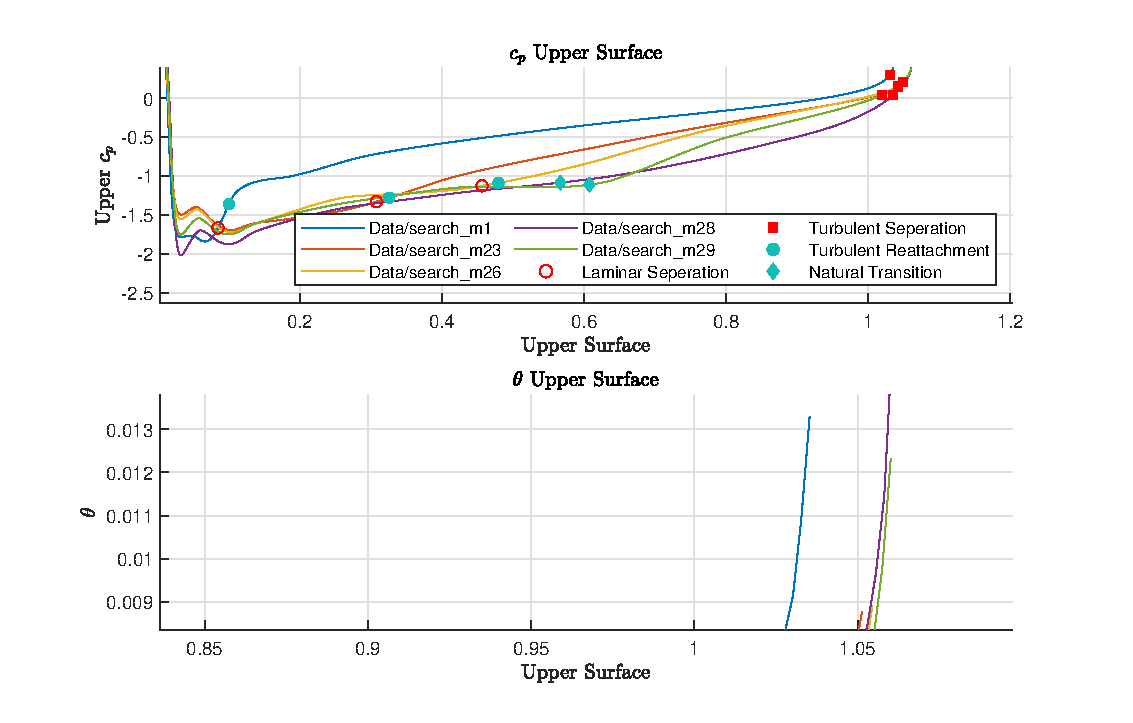
\includegraphics[width=0.99\textwidth]{figures/loRe_upperprofile_29_a5.eps}
        \caption{Pressure coefficient and momentum thickness profiles for $\alpha = 7^\circ$}
        \label{fig:m29_uprofile}
    \end{subfigure}
    \caption{Performance of design iterations 22-29 and their upper surface boundary layer profiles}
\end{figure}

This reduced the pressure on the top surface significantly increasing lift.
Mark 28 shows that the laminar separation bubble was pushed so far back that natural transition occurs instead.
This was expected to significantly reduce the drag, however, turbulent separation was now occurring sooner which increased the drag.
This was found to be due to a stronger adverse pressure gradient at the trailing edge.

Mark 29 featured reduction in curvature at the trailing edge, which delayed transition but produced regions of initially larger, then smaller adverse pressure gradients.
This caused earlier turbulent separation but reduced turbulent boundary layer growth after separation to reach a smaller final momentum thickness, and hence drag.
Another marginal improvement was seen in the final design mark 31. 

\begin{figure}[H]
    \begin{subfigure}{0.54\textwidth}
        \centering
        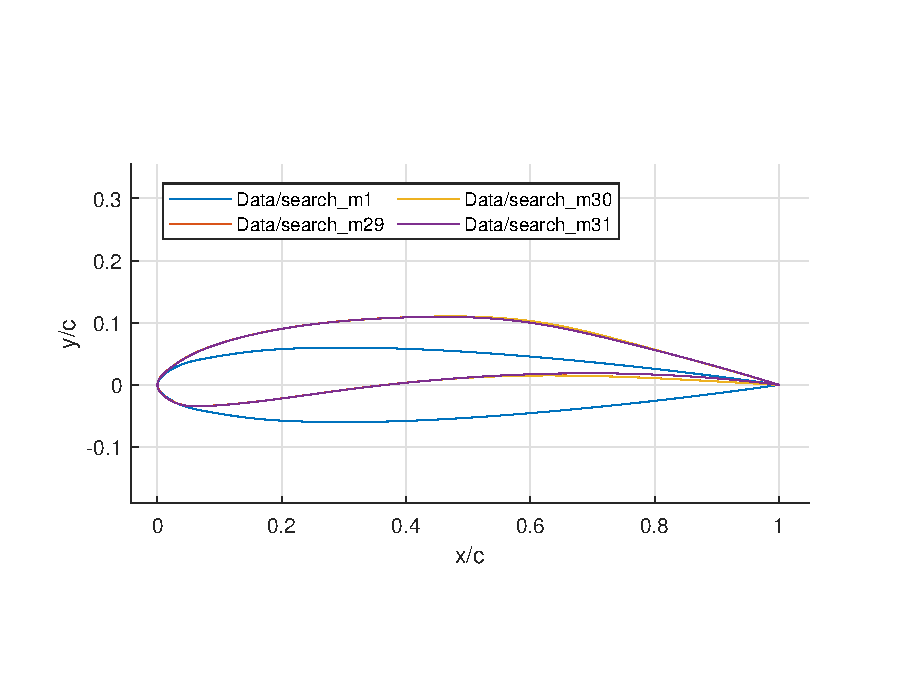
\includegraphics[width=1.2\textwidth, center]{figures/loRe_geometry_31.eps}
        \caption{Airfoil Geometry}
        \label{fig:m31_geometry}
    \end{subfigure}
    \begin{subfigure}{0.45\textwidth}
        \centering
        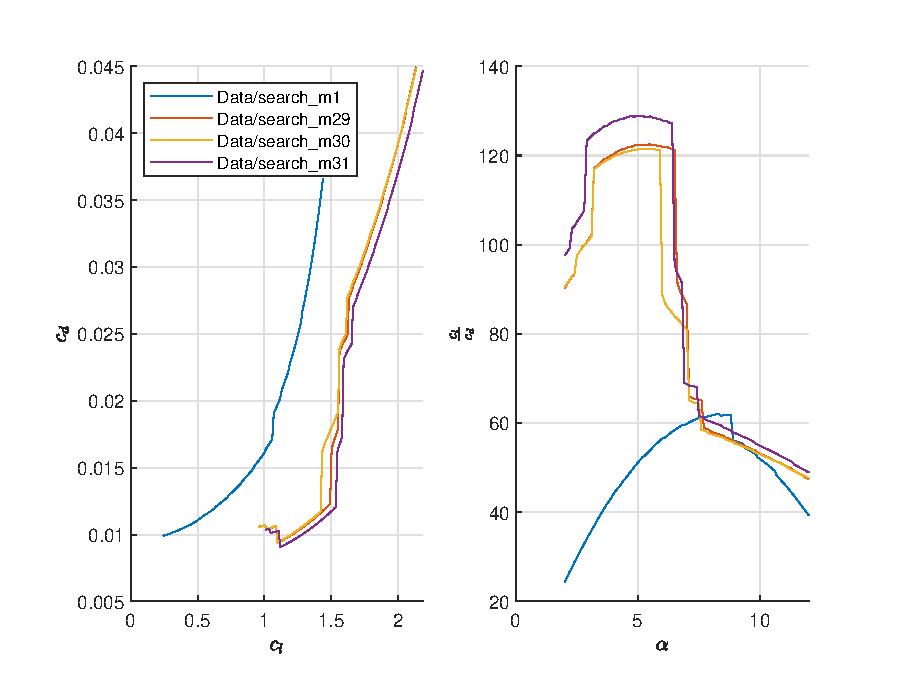
\includegraphics[width=1.2\textwidth, center]{figures/loRe_lod_31.eps}
        \caption{Drag polar and lift to drag ratio against angle of attack}
        \label{fig:m31_lod}
    \end{subfigure}
    \caption{}
\end{figure}

\section{Extensions}

A function was created to calculate the relative change in lift to drag ratio for 0.1\% change in each control point y position.
Figure \ref{fig:ctrl_sensitivity} shows the sensitivity of the control points for our designed aerofoils at their operating Reynolds numbers and $\alpha = 5^\circ$.

\begin{figure}[H]
    \centering
    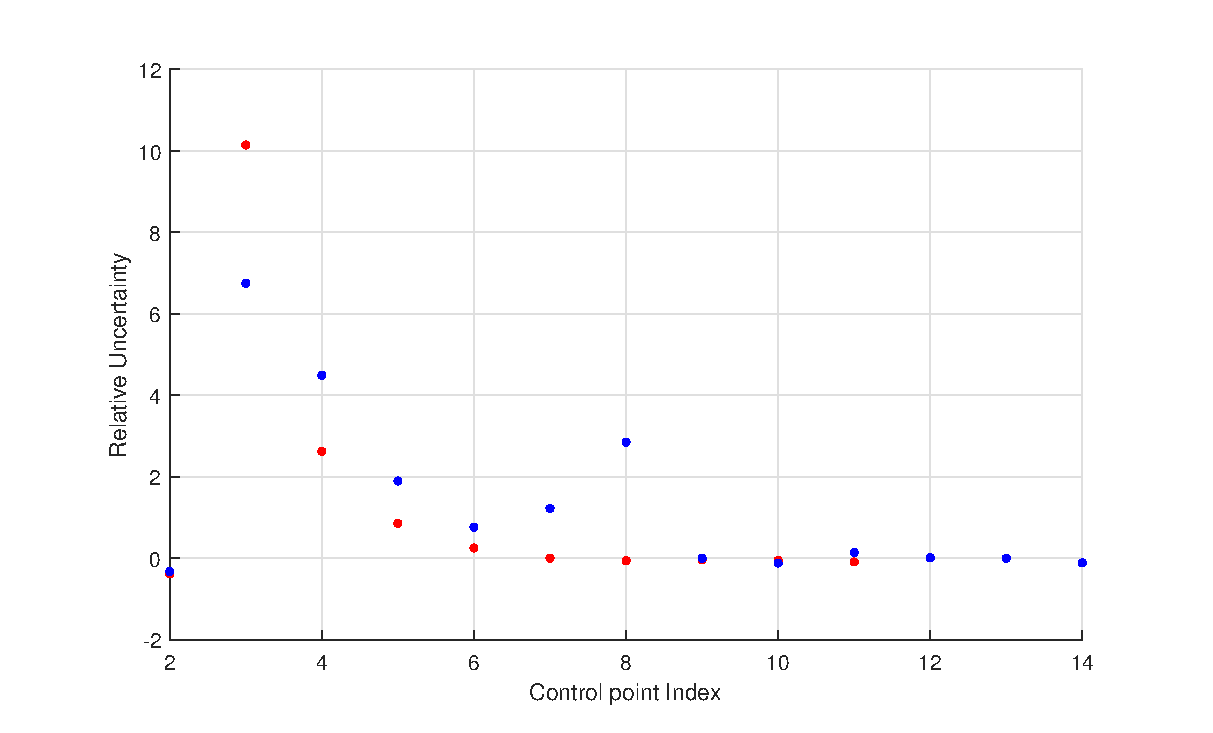
\includegraphics[width=0.8\textwidth]{figures/ctrl_sensitivity.eps}
    \caption{Control point sensitivity analysis. Red indicates version 23 at $Re = 20\times10^6$ and blue indicates mark 31 at $Re = 0.5\times10^6$}
    \label{fig:ctrl_sensitivity}
\end{figure}

This shows that the most sensitive control points are close to the trailing edge.
A 0.1\% increase in the y position of the first upper surface control point from the trailing edge caused the lift to drag ratio to change by ten-fold.
This is unintuitive as it would be expected that the most sensitive control points should be upstream of the boundary layer.
However, the trailing edge applies the Kutta condition which determines the position of the stagnation point, 
which can significantly affect the pressure distribution and boundary layer behaviour.
Its also important to note that the spline control points are highly sensitive and so a relative tolerance of 0.1\% would give a much higher relative tolerance in the surface shape.

\subsection{Vectorized methods}

\begin{figure}[H]
    \centering
    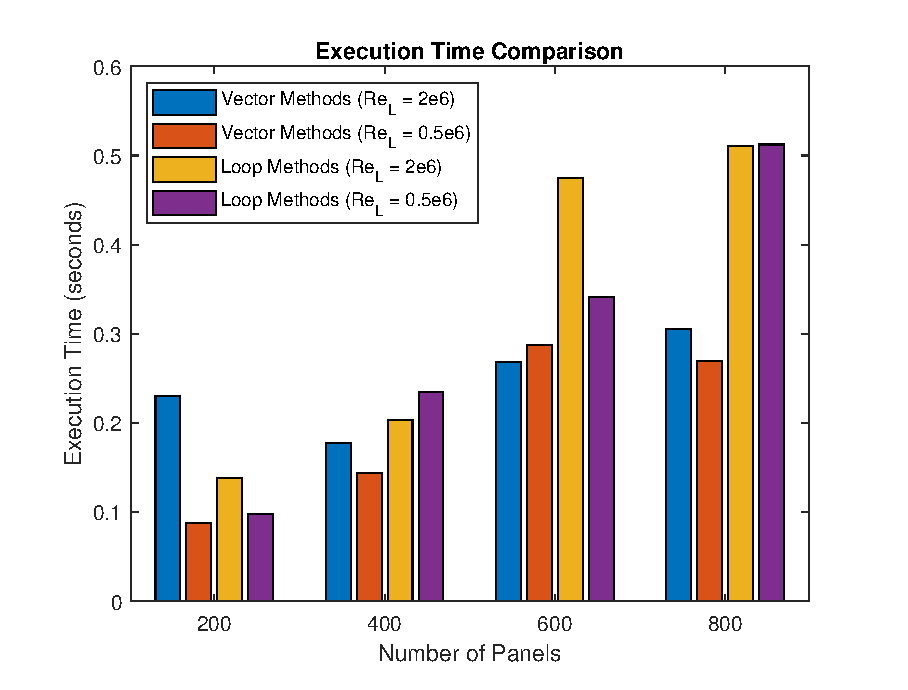
\includegraphics[width=0.6\textwidth]{figures/RePanelVec_times.eps}
    \caption{Computation time for NACA 0012 airfoil for varying number of panels, low and high Reynolds numbers, vectorized and loop algorithms at $\alpha = 5^\circ$}
    \label{fig:RePanelVec_times}
\end{figure}

\subsection{Bezier Spline Optimization}

Instead of manually changing the control points, a Bezier spline can be used to paramaterize the airfoil shape.
The x values of the control points were chosen to be equally spaced along the chord length, and the y values were to be optimised for.
There is a single constraint that the airfoil must not self-intersect.
Additional constraints were partially implemented such as minimum thickness due to the integrated lift bending moment of trailing edge.

It was interesting to note that for many manually selected initial conditions, the optimizer would converge to local maximum lift to drag ratios.
The optimizer was run for a large number of random initial conditions and a global maximum was found at a lift to drag ratio of.

\subsection{Manufacturability}

The aerospace industry is highly regulated, and known for high precision manufacturing.
However, the designs chosen by the software can be extremely sensitive, and so even minor deviations in the manufacturing process could lead to decreased performance.

The software does not account for aeroelastic effects such as wing bending and twisting.
Additional constraints were partially implemented such as minimum thickness due to the integrated lift bending moment of trailing edge.


\begin{thebibliography}{9}
    \bibitem{handout}
    Garcia-Mayoral Ricardo, \textit{Project SA1—Aircraft Wing Analysis Handout} Cambridge University Engineering Department, 2024.

    \bibitem{Eppler_Somers}
    Eppler \& Somers, \textit{A computer program for the design and analysis of low-speed airfoils}, NASA TM 80210.

    \bibitem{BL_notes}
    Li Jie, \textit{3A1: Boundary Layers Handout}. Cambridge University Engineering Department, 2023.
\end{thebibliography}

\end{document}
